%% -------------------------------------------------------------- %%
% 								   %
%                    TEMPLATE DE DOCUMENT LATEX       	           %
%                      Ecole Centrale de Lyon			   %
%             Template LaTeX : Copyright Damien Douteaux           %
%                       Décembre 2016 - Lyon                       %
% 								   %
%% -------------------------------------------------------------- %%


%% -------------------------------------------------------------- %%
%								   %
%                         Type du document			   %
%								   %
%% -------------------------------------------------------------- %%

\documentclass[11pt,a4paper]{article}

%% -------------------------------------------------------------- %%
%								   %
%            Importation des fichiers de configuration             %
%								   %
%% -------------------------------------------------------------- %%

%
% 1 - Fichier d'import des packages
%
%% Global libraries
%\usepackage[top=1.5cm, bottom=1.5cm, outer=5cm, inner=2cm, marginparwidth=2.5cm, marginparsep=.5cm]{geometry}
\usepackage[top=2cm, bottom=2cm, outer=7cm, inner=1.5cm, marginparwidth=5cm, marginparsep=.75cm]{geometry}
\usepackage[french]{babel} % language type annotations

%% Libraries for graphics and colours
\usepackage{tikz} % for drawing
\usepackage{graphicx} % improve include graphics
\usepackage{lipsum} % for testing
\usepackage[most]{tcolorbox} % to have fill paterns for TikZ
\usepackage{changepage} % for adjustwidth command
\usepackage{xcolor} % to have access to every immaginable color
\usepackage{colortbl}
\usepackage{amsmath} % mathematics package
\usepackage{amssymb} % mathematics symbols
\usepackage[explicit,pagestyles]{titlesec} % redefine titles style
\usepackage{mdframed} % permet de couper du texte entre plusieurs pages
\usepackage{framed}
\usepackage{titletoc} % redefine toc
\usepackage{etoolbox} % ?? (used to redefine toc)
\usepackage{stmaryrd}
\usepackage{ifthen} % use to make if then conditions
\usepackage{tikzscale} % in order to scale TikZ pictures
\usepackage{multicol}
\usepackage{capt-of}
\usepackage{xspace}
\usepackage{array}
\usepackage[normalem]{ulem}
\usepackage{url}
\usepackage{subcaption}
\usepackage{cite}
\usepackage{pdftexcmds} % Comparaison de string dans switch case
\usepackage{marginnote}
\usepackage{sidenotes}
\usepackage{lastpage}

%% Other libraries
\usepackage{eurosym} % in order to have € symbol
\usepackage{notoccite} % helps for quotations
\usepackage{float} % helps to place figures
\usepackage[unicode]{hyperref} % in order to make hyperref links inside doc
\usepackage{setspace} % in order to help adding space in the document
\usepackage{longtable} % in order to have multipage tables
\usepackage{multirow} % in order to use multirow in a table
\usepackage{pifont} % in order to have checkmarks and crosses
\usepackage{booktabs} % to have predefined tab rules
\usepackage{rotating} % to have rotating boxes
\usepackage{tkz-tab}
\usepackage{mathrsfs}

%% TikZ libraries needed to compute
\usetikzlibrary{fit} 
\usetikzlibrary{graphs} % package for graphics representation
\usetikzlibrary{positioning} % possitionning inside TikZ picture
\usetikzlibrary{arrows} % beautiful arrows with TikZ
\usetikzlibrary{calc} % enable computation of values insidecture
\usetikzlibrary{decorations} % decoration for TikZ picture

%
% 2 - Fichier de configuration utilisateur
%
\definecolor{themeColor}{RGB}{199,16,26}
\definecolor{vertforet}{RGB}{20,83,20}
\definecolor{bordeau}{RGB}{199,16,26}
\definecolor{gris}{RGB}{195,195,195}
\definecolor{bluenight}{RGB}{0,82,148}
\definecolor{bluesword}{RGB}{0,82,148}
\definecolor{violet}{RGB}{112,4,98}
\definecolor{amber}{RGB}{255,110,0}
\definecolor{mygray}{RGB}{125,125,125}

\newcommand{\currentColor}{themeColor}
\newcommand{\headersColor}{themeColor}
%\def \currentColor {themeColor}
\newcommand\thColor[1]{\textcolor{themeColor}{#1}}
\newcommand\curColor[1]{\textcolor{\currentColor}{#1}}
\newcommand\headColor[1]{\textcolor{\headersColor}{#1}}
\newcommand\wiColor[1]{\textcolor{white}{#1}}

%%% Local Variables:
%%% mode: plain-tex
%%% TeX-master: "../Master"
%%% End:

%%---------------------------------------------------------------%%
%                                                                 %
%   Fichier de toutes les configurations basiques utilisateurs    %
%                                                                 %
%%---------------------------------------------------------------%%

%
% 1 - Positionnement des TOC - LOF - LOT dans le document
%
\newcommand\whereTOC{beginning}          % Parmis beginning - end
\newcommand\whereLOF{end}                % Parmis beginning - end
\newcommand\whereLOT{end}                % Parmis beginning - end
\newcommand\TOCLOFTNumStyle{Roman}       % Parmis Roman - roman - Arabic - arabic
\newcommand\LOFLOTSeparator{\vfill}      % Séparateur après une LOF ou LOT
\newcommand\TOCSeparator{\newpage}       % Séparateur après un TOC
\newcommand\inclureTOC{true}             % Mettre la TOC (true) ou pas (false)
\newcommand\inclureLOF{false}            % Mettre la LOF (true) ou pas (false)
\newcommand\inclureLOT{false}            % Mettre la LOT (true) ou pas (false)

%
% 2 - Fichiers à inclure
%
\newcommand\inclureIntroduction{false}   % Mettre l'introduction (true) ou pas (false)    -> Position imposée
\newcommand\inclureConclusion{false}     % Mettre la conclusion (true) ou pas (false)     -> Position imposée
\newcommand\inclureRemerciements{false}  % Mettre les remerciements (true) ou pas (false)
\newcommand\inclureResume{false}         % Mettre le résumé (true) ou pas (false)
\newcommand\inclureAbstract{false}       % Mettre le résumé anglais (true) ou pas (false)
\newcommand\inclureReferences{false}     % Mettre les références (true) ou pas (false)
\newcommand\whereResume{beginning}       % Parmis beginning - end
\newcommand\whereRemerciements{beginning}% Parmis beginning - end
\newcommand\whereReferences{end}         % Parmis beginning - end

%
% 3 - Informations pour en-têtes et pieds de page
%
\newcommand\footerRight{\textbf{Année 2017}   }                    % À gauche séparation du footer
\newcommand\footerLeft{\textbf{\thepage}}                          % À droite séparation du footer
\newcommand\headerText{\textbf{Principe et applications de XGBoost}}   % Texte de l'en-tête
\newcommand\headerLogo{logo}                                       % Logo de l'en-tête (optionnel)

%
% 4 - Page de titre à charger
%
\newcommand\titlePage{picture}                                     % Voir les noms dans conf/Pages_titre/

%
% 5 - Le type de sections désiré
%

% 5.1 - Aspect d'une partie
\newcommand\partFormat{page}
\newcommand\partModele{default}
% 5.2 - Aspect d'une section
\newcommand\sectionFormat{greatNumber}
\newcommand\sectionNumber{arabic}
\newcommand\sectionNumberStyle{textbfgray}
\newcommand\sectionSeparator{}
\newcommand\sectionSeparatorStyle{thColor}
\newcommand\sectionTextStyle{textbfc}
% 5.3 - Aspect d'une sous-section
\newcommand\subsectionFormat{light}
\newcommand\subsectionNumber{arabic}
\newcommand\subsectionNumberStyle{textbfc}
\newcommand\subsectionSeparator{~~$\bullet$~~}
\newcommand\subsectionSeparatorStyle{thColor}
\newcommand\subsectionTextStyle{thColor}
% 5.4 - Aspect d'une sous-sous-section
\newcommand\subsubsectionFormat{default}
\newcommand\subsubsectionNumber{arabic}
\newcommand\subsubsectionNumberStyle{thColor}
\newcommand\subsubsectionSeparator{~~}
\newcommand\subsubsectionSeparatorStyle{textbf}
\newcommand\subsubsectionTextStyle{textit}
% 5.5 - Aspect d'un paragraphe
\newcommand\paragrapheFormat{default}
\newcommand\paragrapheNumber{none}        % Pas de numérotation (none), autrement {Roman ; roman ; arabic ; Arabic}
\newcommand\paragrapheNumberStyle{}
\newcommand\paragrapheSeparator{}
\newcommand\paragrapheSeparatorStyle{}
\newcommand\paragrapheTextStyle{}
% 5.6 - Aspect d'un sous-paragraphe
\newcommand\subparagrapheFormat{default}
\newcommand\subparagrapheNumber{none}     % Pas de numérotation (none), autrement {Roman ; roman ; arabic ; Arabic}
\newcommand\subparagrapheNumberStyle{}
\newcommand\subparagrapheSeparator{}
\newcommand\subparagrapheSeparatorStyle{}
\newcommand\subparagrapheTextStyle{textic}
% 5.7 - Aspect de la page d'annexe
\newcommand\annexeModele{default}         % Aucune (none) ou voir dans conf/Pages_annexes/

%
% 6 - Pour les sections avec images, configuration des images
%
\newcommand\imageSectionI{default1}
\newcommand\imageSectionII{default2}
\newcommand\imageSectionIII{default3}
\newcommand\imageSectionIV{default4}
\newcommand\imageSectionV{default5}
%%---------------------------------------------------------------%%
%                                                                 %
%       !!! NE PAS CHANGER SAUF SI ON SAÎT CE QU'ON FAIT !!!      %
%      Inclusions automatiques en fonction des configurations     %
%                                                                 %
%%---------------------------------------------------------------%%

% 1 - La page de garde
\input{conf/Pages_garde/page_garde__\titlePage}       % Charger les configurations de cette page titre

% 2 - La page d'aspect de partie
\input{conf/Pages_parties/part__\partModele}    % Charger les configurations du bon modèle de page pour les parties

% 3 - La page d'aspect des annexes
\input{conf/Pages_annexes/annexe__\annexeModele}  % Charger les configurations du bon modèle de page pour les parties

%
% 3 - Fichier de définition des styles
%
%
% Méthode pour l'inclusion automatique de fichier/élément à l'endroit désiré
% Params :
%     1 - Elément à inclure
%     2 - Configuration pour le choix (\whereXXX)
%     3 - Endroit à tester
%     4 - S'il y a possibilité de ne pas inclure l'élément
%
\makeatletter
\newcommand{\whereIncludeFile}[4]{
  \ifnum\pdf@strcmp{#4}{true}=0
  \ifnum\pdf@strcmp{#2}{#3}=0
  #1
  \fi\fi
}
\makeatother

\newcommand{\includeTOC}[1]{
  \whereIncludeFile{\clearpage\tableofcontents\TOCSeparator}{\whereTOC}{#1}{\inclureTOC}
}

\newcommand{\includeLOF}[1]{
  \whereIncludeFile{\listoffigures\LOFLOTSeparator}{\whereLOF}{#1}{\inclureLOF}
}

\newcommand{\includeLOT}[1]{
  \whereIncludeFile{\listoftables\LOFLOTSeparator}{\whereLOT}{#1}{\inclureLOT}
}

\newcommand{\includeResume}[1]{
  \whereIncludeFile{\nnsection{Résumé}
Ceci est le résumé du document

\begin{figure}[ht]
  \caption{Une figure magnifique}
  \label{fig:mafig}
\end{figure}

\begin{table}[ht]
  \caption{Un tableau vital pour la suite}
  \label{tab:vital}
\end{table}


%%% Local Variables:
%%% mode: latex
%%% TeX-master: "../../Template"
%%% End:
}{\whereResume}{#1}{\inclureResume}
}

\newcommand{\includeAbstract}[1]{
  \whereIncludeFile{\input{text/Pages_gnl/abstract.tex}}{\whereResume}{#1}{\inclureAbstract}
}

\newcommand{\includeRemerciements}[1]{
  \whereIncludeFile{\input{text/Pages_gnl/remerciements.tex}}{\whereRemerciements}{#1}{\inclureRemerciements}
}

\newcommand{\includeIntroduction}{
  \whereIncludeFile{\nnsection{Introduction}
\label{sec:introduction}
L'introduction du document

%%% Local Variables:
%%% mode: latex
%%% TeX-master: "../../Rapport_RO_BE1"
%%% End:
}{beginning}{beginning}{\inclureIntroduction}
}

\newcommand{\includeConclusion}{
  \whereIncludeFile{\nnsection{Conclusion}

%%% Local Variables:
%%% mode: latex
%%% TeX-master: "../../Rapport_dreches"
%%% End:
}{beginning}{beginning}{\inclureConclusion}
}

%
% Afficher un argument si l'autre est non vide
% Params :
%     1 - Texte à afficher
%     2 - Valeur de contrôle
%
%\newcommand{\printIfNotZero}[2]{
%  \ifnum#2=0
%  \else
%  #1
%  \fi
%}
\newcommand{\printIfNotZero}[2]{%
  \ifthenelse{#2=0}{}{#1}%
}

%%% Local Variables:
%%% mode: latex
%%% TeX-master: "../Template"
%%% End:

%
% Applique un formatage sur le texte fourni
% Params :
%     1 - Le format demandé
%     2 - Le texte à mettre en forme
%
\makeatletter
\newcommand{\applyFormat}[2]{%
  \ifnum\pdf@strcmp{#1}{textbi}=0%
  \textbi{#2}%
  \else\ifnum\pdf@strcmp{#1}{textbf}=0%
  \textbf{#2}%
  \else\ifnum\pdf@strcmp{#1}{textit}=0%
  \textit{#2}%
  \else\ifnum\pdf@strcmp{#1}{textsc}=0%
  \textsc{#2}%
  \else\ifnum\pdf@strcmp{#1}{textbic}=0%
  \textbic{#2}%
  \else\ifnum\pdf@strcmp{#1}{textbfc}=0%
  \textbfc{#2}%
  \else\ifnum\pdf@strcmp{#1}{textic}=0%
  \textic{#2}%
  \else\ifnum\pdf@strcmp{#1}{textscic}=0%
  \textbic{#2}%
  \else\ifnum\pdf@strcmp{#1}{textscc}=0%
  \textscc{#2}%
  \else\ifnum\pdf@strcmp{#1}{thColor}=0%
  \thColor{#2}%
  \else\ifnum\pdf@strcmp{#1}{textbfgray}=0%
  \textbfgray{#2}%
  \fi\fi\fi\fi\fi\fi\fi\fi\fi\fi\fi%
}
\makeatother

\newcommand\textbi[1]{%
  \textbf{\textit{#1}}%
}

\newcommand\textbic[1]{%
  \textbf{\textit{\thColor{#1}}}%
}

\newcommand\textbfc[1]{%
  \textbf{\thColor{#1}}%
}

\newcommand\textbfgray[1]{%
  \textbf{\textcolor{gray}{#1}}%
}

\newcommand\textscic[1]{%
  \textsc{\textit{\thColor{#1}}}%
}

\newcommand\textscc[1]{%
  \textsc{\thColor{#1}}%
}

\newcommand\textic[1]{%
  \textit{\thColor{#1}}%
}
  

%%% Local Variables:
%%% mode: latex
%%% TeX-master: "../Template"
%%% End:

% Some pre-defined TikZstyles
\tikzset{
	sectionleft/.style={text height=1.5ex,text depth=0ex,color=\headersColor},
	drawrect/.style={draw, rectangle, fill=#1},
	footers/.style={draw, rectangle, minimum width=21cm, minimum height = 0.5cm, color=#1, fill=#1},
	headers/.style={draw, rectangle, minimum width=21cm, minimum height = 0.5cm, color=#1, fill=#1},
	headers/.default=\headersColor,
	footers/.default=\headersColor,
	drawrect/.default=\headersColor,
    rectangle with rounded corners north west/.initial=4pt,
    rectangle with rounded corners south west/.initial=4pt,
    rectangle with rounded corners north east/.initial=4pt,
    rectangle with rounded corners south east/.initial=4pt
}

\pgfdeclarelayer{background}
\pgfdeclarelayer{foreground}
\pgfsetlayers{background,main,foreground}

\makeatletter
\pgfdeclareshape{rectangle with rounded corners}{
  \inheritsavedanchors[from=rectangle] % this is nearly a rectangle
  \inheritanchorborder[from=rectangle]
  \inheritanchor[from=rectangle]{center}
  \inheritanchor[from=rectangle]{north}
  \inheritanchor[from=rectangle]{south}
  \inheritanchor[from=rectangle]{west}
  \inheritanchor[from=rectangle]{east}
  \inheritanchor[from=rectangle]{north east}
  \inheritanchor[from=rectangle]{south east}
  \inheritanchor[from=rectangle]{north west}
  \inheritanchor[from=rectangle]{south west}
  \backgroundpath{% this is new
    % store lower right in xa/ya and upper right in xb/yb
    \southwest \pgf@xa=\pgf@x \pgf@ya=\pgf@y
    \northeast \pgf@xb=\pgf@x \pgf@yb=\pgf@y
    % construct main path
    \pgfkeysgetvalue{/tikz/rectangle with rounded corners north west}{\pgf@rectc}
    \pgfsetcornersarced{\pgfpoint{\pgf@rectc}{\pgf@rectc}}
    \pgfpathmoveto{\pgfpoint{\pgf@xa}{\pgf@ya}}
    \pgfpathlineto{\pgfpoint{\pgf@xa}{\pgf@yb}}
    \pgfkeysgetvalue{/tikz/rectangle with rounded corners north east}{\pgf@rectc}
    \pgfsetcornersarced{\pgfpoint{\pgf@rectc}{\pgf@rectc}}
    \pgfpathlineto{\pgfpoint{\pgf@xb}{\pgf@yb}}
    \pgfkeysgetvalue{/tikz/rectangle with rounded corners south east}{\pgf@rectc}
    \pgfsetcornersarced{\pgfpoint{\pgf@rectc}{\pgf@rectc}}
    \pgfpathlineto{\pgfpoint{\pgf@xb}{\pgf@ya}}
    \pgfkeysgetvalue{/tikz/rectangle with rounded corners south west}{\pgf@rectc}
    \pgfsetcornersarced{\pgfpoint{\pgf@rectc}{\pgf@rectc}}
    \pgfpathclose
 }
}
\makeatother

%%% Local Variables:
%%% mode: plain-tex
%%% TeX-master: "../Master"
%%% End:

%%  boxing (general code)
\newcommand\generalencadrement[5]{\renewcommand{\currentColor}{#3}\vspace{0.3cm}\noindent\tikz{[line width=1]
\node (contentnode) [draw, color=#3, fill=#4, text=black, rectangle, inner sep = 15, outer sep = 0, rounded corners = 2mm, minimum width=\linewidth-1, text width=\linewidth-31,align=justify, right] at (0,0) {\newline #2};
\node [draw,rectangle,inner sep = 3,outer sep = 3,rounded corners = 1mm, fill opacity=1, above, color=#3, fill=#5, text =black, right]  at ([xshift=15]contentnode.north west) {\hspace{0.1cm}#1 \hspace{0.1cm}};
}\par\vspace{0.3cm}\renewcommand{\currentColor}{themeColor}}

\newcommand\customgeneralencadrement[5]{\vspace{.15cm}\begin{tcolorbox}[breakable, title={#1}, attach boxed title to top left= {xshift=10mm,yshift=-3mm}, boxed title style={boxrule=.8pt}, colframe=#3, colback=#5, coltitle=black, colbacktitle=#4, boxrule=.8pt]
\vspace{.3cm}
#2
\end{tcolorbox}}

%% Several types of useful boxes (using previous source code)
\newcommand\remarqueencadr[1]{\par\generalencadrement{ Remark }{ #1 }{vertforet}{white}{white}}
\newcommand\attentionencadr[1]{\par\generalencadrement{ Beware }{ #1 }{bordeau}{white}{white}}
\newcommand\informationencadr[1]{\par\generalencadrement{ Information }{ #1 }{orange}{white}{white}}
\newcommand\paragrapheencadr[2]{\par\generalencadrement{ #1 }{ #2 }{themeColor}{white}{white}}

\newcommand\remarqueencadrfond[1]{\par\generalencadrement{ Remark }{ #1 }{vertforet}{vertforet!50}{white}}
\newcommand\attentionencadrfond[1]{\par\generalencadrement{ Beware }{ #1 }{bordeau}{bordeau!50}{white}}
\newcommand\informationencadrfond[1]{\par\generalencadrement{ Information }{ #1 }{orange}{orange!50}{white}}
\newcommand\paragrapheencadrfond[2]{\par\generalencadrement{ #1 }{ #2 }{themeColor}{themeColor!50}{white}}

\newcommand\remarqueencadrfondd[1]{\par\generalencadrement{ Remark }{ #1 }{vertforet}{vertforet!5}{vertforet!50}}
\newcommand\attentionencadrfondd[1]{\par\generalencadrement{ Beware }{ #1 }{bordeau}{bordeau!5}{bordeau!50}}
\newcommand\informationencadrfondd[1]{\par\generalencadrement{ Information }{ #1 }{orange}{orange!5}{orange!50}}
\newcommand\paragrapheencadrfondd[2]{\par\generalencadrement{ #1 }{ #2 }{themeColor}{themeColor!5}{themeColor!50}}

\newcommand\mathdefinition[2]{\par\generalencadrement{ Definition --- #1 }{ #2 }{bluenight}{white}{white}}
\newcommand\mathdefinitionvoid[1]{\par\generalencadrement{ Definition }{ #1 }{bluenight}{white}{white}}
\newcommand\maththeoreme[2]{\par\generalencadrement{ Theorem --- #1 }{ #2 }{vertforet}{white}{white}}
\newcommand\maththeoremevoid[1]{\par\generalencadrement{ Theorem }{ #1 }{vertforet}{white}{white}}
\newcommand\mathpropriete[2]{\par\generalencadrement{ Propriety --- #1 }{ #2 }{orange}{white}{white}}
\newcommand\mathproprietevoid[1]{\par\generalencadrement{ Propriété }{ #1 }{orange}{white}{white}}
\newcommand\mathcasparticulier[2]{\par\generalencadrement{ Particular case --- #1 }{ #2 }{violet}{white}{white}}
\newcommand\mathcasparticuliervoid[1]{\par\generalencadrement{ Particular case }{ #1 }{violet}{white}{white}}
\newcommand\mathmethode[2]{\par\generalencadrement{ Method --- #1 }{ #2 }{bordeau}{white}{white}}
\newcommand\mathexercice[2]{\par\generalencadrement{ Exercise #1 }{ #2 }{bluenight}{white}{white}}
\newcommand\mathenonce[1]{\par\generalencadrement{ Problem statement }{ #1 }{bluenight}{white}{white}}
\newcommand\mathproposition[2]{\par\generalencadrement{ Proposition --- #1 }{ #2 }{orange}{white}{white}}
\newcommand\mathpropositionvoid[1]{\par\generalencadrement{ Proposition }{ #1 }{orange}{white}{white}}

%% Boxes to enhanced results
\newcommand{\result}[1]{\tresult{$\displaystyle{#1}$}}
\newcommand{\tresult}[1]{\colorbox{themeColor!30}{#1}}

%%% Local Variables:
%%% mode: latex
%%% TeX-master: "../Master"
%%% End:

%% Rededefining table of contents
\addto\captionsfrench{ % French stands for the used language
  \renewcommand{\contentsname}{En~bref}%
  \renewcommand{\listfigurename}{Liste des figures}%
  \renewcommand{\listtablename}{Liste des tables}%
}

\setcounter{tocdepth}{1}

\makeatletter
%% Style des sections dans la TOC
\titlecontents{section}[0mm]% partial section style
{\contentsmargin[4mm]{0mm}\fontspec{Fira Sans Book}\alignLeftOrRightStandaloneInversed\small}%
{\thColor{$\blacktriangleright$}\hspace*{6pt}(p.\hspace*{3pt}\thecontentspage)\hspace*{6pt}}%
{}%
{}{}%

\makeatletter
\renewcommand\tableofcontents{%
  \textbf{\Large\contentsname}\hfill\rule{0pt}{0pt}\newline\thColor{\rule{\textwidth}{2pt}}\newline\par
  \@mkboth{\MakeUppercase\contentsname}{\MakeUppercase\contentsname}%
  \@starttoc{toc}%
}
\makeatother
%% Caption package
%\usepackage{caption}
\DeclareCaptionLabelSeparator{bullet}{~\headColor{$\bullet$}~}
\captionsetup{labelfont={bf,color=\headersColor},labelsep=bullet}
\DeclareCaptionStyle{sidecaption}{labelfont={bf,color=\headersColor},labelsep=bullet}
%% Defining our itemize bullet
\newcommand\mybullet{\tikz{\draw [color=\currentColor, fill=\currentColor] (0,0) circle [radius=.03cm]; \draw [color=\currentColor,thick] (0,0) circle [radius=0.1cm];}}

\newcommand\itemperso[1]{\item[\mybullet]~\textit{\textcolor{\currentColor}{#1}}\ifthenelse{\equal{#1}{}}{}{\hspace{0.5cm}}}

\newcommand{\tabitem}{~~\llap{\mybullet}~~}

\newcommand\subitemperso[1]{\item[\textcolor{\currentColor}{$\triangleright$}] \textit{\textcolor{\currentColor}{#1}}\ifthenelse{\equal{#1}{}}{}{\hspace{0.2cm}}}

\newcommand\subsubitemperso[1]{\item[\textcolor{\currentColor}{$\star$}] \textit{\textcolor{\currentColor}{#1}}\ifthenelse{\equal{#1}{}}{}{\hspace{0.2cm}}}

%% New items for school work questions
\newcommand\exquestion[1]{\vspace{.1cm}\item[\mybullet] \textcolor{\currentColor}{#1}\ifthenelse{\equal{#1}{}}{}{\hspace{0.5cm}}}

\newcommand\exsubquestion[1]{\item[\textcolor{\currentColor}{$\triangleright$}] \textcolor{\currentColor}{#1}\ifthenelse{\equal{#1}{}}{}{\hspace{0.2cm}}}

\newcommand\exsubsubquestion[1]{\item[\textcolor{\currentColor}{$\star$}] \textcolor{\currentColor}{#1}\ifthenelse{\equal{#1}{}}{}{\hspace{0.2cm}}}

%% Commands to define tick, cross and neutral mark
\newcommand{\cmark}{\textcolor{vertforet}{\ding{51}}}%
\newcommand{\xmark}{\textcolor{bordeau}{\ding{55}}}%
\newcommand{\neutral}{\textcolor{gray}{\ding{70}}}%
\newcommand\testStatus[1]{\ifthenelse{\equal{#1}{OK}}{\cmark}{\ifthenelse{\equal{#1}{NSP}}{\neutral}{\xmark}}}

\newcommand\itemtest[3]{\itemperso{}\begin{minipage}[t]{\dimexpr\linewidth-.5cm\relax}%
	\textit{\textcolor{themeColor}{#1}}\ifthenelse{\equal{#1}{}}{}{\hspace{0.5cm}}#2\end{minipage}%
	\hspace{\fill}\testStatus{#3}}
\newcommand\subitemtest[3]{\subitemperso{}\begin{minipage}[t]{\dimexpr\linewidth-.5cm\relax}%
	\textit{\textcolor{themeColor}{#1}}\ifthenelse{\equal{#1}{}}{}{\hspace{0.5cm}}#2\end{minipage}%
	\hspace{\fill}\testStatus{#3}}
\newcommand\subsubitemtest[3]{\subsubitemperso{}\begin{minipage}[t]{\dimexpr\linewidth-.5cm\relax}
	\textit{\textcolor{themeColor}{#1}}\ifthenelse{\equal{#1}{}}{}{\hspace{0.5cm}}#2\end{minipage}%
	\hspace{\fill}\testStatus{#3}}

\newcommand\itemtestdouble[4]{\itemperso{}\begin{minipage}[t]{\dimexpr\linewidth-1cm\relax}%
	\textit{\textcolor{themeColor}{#1}}\ifthenelse{\equal{#1}{}}{}{\hspace{0.5cm}}#2\end{minipage}%
	\hspace{\fill}\testStatus{#3}\hspace{\fill}\testStatus{#4}}
\newcommand\subitemtestdouble[4]{\subitemperso{}\begin{minipage}[t]{\dimexpr\linewidth-1cm\relax}%
	\textit{\textcolor{themeColor}{#1}}\ifthenelse{\equal{#1}{}}{}{\hspace{0.5cm}}#2\end{minipage}%
	\hspace{\fill}\testStatus{#3}\hspace{\fill}\testStatus{#4}}
\newcommand\subsubitemtestdouble[4]{\subsubitemperso{}\begin{minipage}[t]{\dimexpr\linewidth-1cm\relax}
	\textit{\textcolor{themeColor}{#1}}\ifthenelse{\equal{#1}{}}{}{\hspace{0.5cm}}#2\end{minipage}%
	\hspace{\fill}\testStatus{#3}\hspace{\fill}\testStatus{#4}}

\newcommand\itemtesttriple[5]{\itemperso{}\begin{minipage}[t]{\dimexpr\linewidth-1.5cm\relax}%
	\textit{\textcolor{themeColor}{#1}}\ifthenelse{\equal{#1}{}}{}{\hspace{0.5cm}}#2\end{minipage}%
	\hspace{\fill}\testStatus{#3}\hspace{\fill}\testStatus{#4}\hspace{\fill}\testStatus{#5}}
\newcommand\subitemtesttriple[5]{\subitemperso{}\begin{minipage}[t]{\dimexpr\linewidth-1.5cm\relax}%
	\textit{\textcolor{themeColor}{#1}}\ifthenelse{\equal{#1}{}}{}{\hspace{0.5cm}}#2\end{minipage}%
	\hspace{\fill}\testStatus{#3}\hspace{\fill}\testStatus{#4}\hspace{\fill}\testStatus{#5}}
\newcommand\subsubitemtesttriple[5]{\subsubitemperso{}\begin{minipage}[t]{\dimexpr\linewidth-1.5cm\relax}
	\textit{\textcolor{themeColor}{#1}}\ifthenelse{\equal{#1}{}}{}{\hspace{0.5cm}}#2\end{minipage}%
	\hspace{\fill}\testStatus{#3}\hspace{\fill}\testStatus{#4}\hspace{\fill}\testStatus{#5}}


\newcommand\testLabels{\noindent\hspace*{\dimexpr\linewidth-1.3cm\relax}\rule{1.3cm}{.4pt}\par\noindent\hspace*{\dimexpr\linewidth-1.3cm\relax}\textbf{V}\hspace{\fill}\textbf{S}\hspace{\fill}\textbf{M}\par\noindent\hspace*{\dimexpr\linewidth-1.3cm\relax}\rule[0.66\baselineskip]{1.3cm}{.4pt}}

%%% Local Variables:
%%% mode: latex
%%% TeX-master: "../Rapport_metro"
%%% End:

%% New headers and footers

\newcommand{\printheaderLeft}{\tikz{%
    \node (header_logo) [text depth=0] at (0,0) {\includegraphics[height=0.55cm]{images/Logo/\headerLogo}};%
    \node (header_text) [right, text depth=0] at ([xshift=1cm]header_logo.east) {\headColor{\headerText}};%
    \fill [\headersColor] ([xshift=.45cm]header_logo.south east) rectangle ([xshift=-.45cm]header_text.north west);%
  }
}

\newcommand{\printheaderRight}{\tikz{%
    \node (header_text) [text depth=0] at (0,0) {\headColor{\headerText}};%
    \node (header_logo) [right, text depth=0] at ([xshift=1cm]header_text.east) {\includegraphics[height=0.55cm]{images/Logo/\headerLogo}};%
    \fill [\headersColor] ([xshift=.45cm]header_text.south east) rectangle ([xshift=-.45cm]header_logo.north west);%
  }
}

\newcommand{\printfooterRight}{\tikz{%
    \node (footer_text) [text depth=0] at (0,0) {\headColor{\footerLeft}};%
    \node (footer_nb_page) [right, text depth=0] at ([xshift=1cm]footer_text.east) {\headColor{\footerRight}};%
    \fill [\headersColor] ([xshift=.45cm]footer_text.south east) rectangle ([xshift=-.45cm]footer_nb_page.north west);%
  }
}

\newcommand{\printfooterLeft}{\tikz{%
    \node (footer_nb_page) [text depth=0] at (0,0) {\headColor{\footerRight}};%
    \node (footer_text) [right, text depth=0] at ([xshift=1cm]footer_nb_page.east) {\headColor{\footerLeft}};%
    \fill [\headersColor] ([xshift=.45cm]footer_nb_page.south east) rectangle ([xshift=-.45cm]footer_text.north west);%
  }
}
  
\makeatletter
\def\ps@mystyle{%
  % Le pied de page des pages du document
  \def\@oddfoot{%
    \ifodd\value{page}\relax%
    \printfooterLeft\hfill
    \else
    \hfill\printfooterRight
    \fi
  }
  % L'en-tête des pages du document
  \def\@oddhead{%
    \ifodd\value{page}\relax
    \printheaderLeft\hfill
    \else
    \hfill\printheaderRight
    \fi%
  }%
  \let\@mkboth\markboth}
\makeatother
\pagestyle{mystyle}
%\tocloftpagestyle{mystyle}


%% Configurations de base pour les liens hyperref
\hypersetup{hidelinks,
		pdfauthor={Damien Douteaux}, 
	        pdftitle={Projet de recherche et développement},
		pdfkeywords={Centrale Lyon, IRD, Projet}}

%% Change margins environment
\def\changemargin#1#2{\list{}{\rightmargin#2\leftmargin#1}\item[]}
\let\endchangemargin=\endlist 

%% Sections needing completion ands type of completions expected
\newcommand{\needCompletion}[1]{\newline\textcolor{purple}{\textit{#1}}\newline}

%% Emphasing elements in a table
\newcommand{\emphasizeTab}{\textcolor{bordeau}{\up{$\circledast$}}}

%% Glossary entry
\newcommand{\itemGlossaire}[3]{\par\textcolor{themeColor}{\textbf{#1}}\label{#2}\hspace{0.7cm}{#3}\vspace{0.2cm}}
\newcommand{\itemAcro}[4]{\par\textcolor{themeColor}{\textbf{#1} (#2)}\label{#3}\hspace{0.7cm}{#4}\vspace{0.2cm}}

%% Other unused commands
\newcommand\roundboxwithline[2]{\noindent\tikz{[line width=1]
\coordinate (leftshift) at (0,0);
\node (sectionname) [draw,rectangle,inner sep = 5,outer sep = 0,rounded corners = 1mm,font=\fontsize{#1}{1}\it\selectfont,color=themeColor,text opacity = 1,right] at (1,0) {#2};
\draw [color=themeColor] (leftshift) -- (sectionname.west);
\draw [color=themeColor] (sectionname.east) -- (\linewidth-1,0);}} 

%% Table interline value
\renewcommand*\arraystretch{1.5}

%% Don't forget me mark
\newcommand\beware{\up{\textcolor{bordeau}{(!)}}}

%% Rectif indices
\newcommand{\rectif}{\hspace{0.05cm}}

%% Special include when newpage is needed
\newcommand{\inputn}[1]{\newpage\input{#1}}

%% Mise en avant de résultats intermédiaires
\newcommand{\iResult}[2]{\iiResult{Intermediate outcome :}{#1}{passengers/#2}{!25}}
\newcommand{\itResult}[2]{\iiResult{Intermediate outcome :}{#1}{trips/#2}{!25}}

\newcommand{\isResult}[3]{\newline\vskip\hspace*{\fill}\large{\textcolor{themeColor}{#1} $#2$ #3}\hspace*{\fill}\newline}

\newcommand{\iiResult}[4]{\newline\vskip\noindent\hspace*{\fill}\colorbox{themeColor}{\rule{0cm}{1cm}\hspace{.07cm}}\colorbox{themeColor#4}{\hspace{.1cm}\rule{0cm}{1cm}\raisebox{.3cm}{\large{\textcolor{themeColor}{#1} $#2$ #3\hspace{.1cm}}}}\hspace*{\fill}}

\newcommand{\qpays}{$\mathcal{Q}_\textnormal{pays}$}
\newcommand{\qvolprod}{$\mathcal{Q}_\textnormal{volume production}$}
\newcommand{\qprofil}{$\mathcal{Q}_\textnormal{profil}$}
\newcommand{\qinteret}{$\mathcal{Q}_\textnormal{aspect important}$}
\newcommand{\qpayback}{$\mathcal{Q}_\textnormal{payback}$}
\newcommand{\qbudget}{$\mathcal{Q}_\textnormal{budget}$}
\newcommand{\qagriculture}{$\mathcal{Q}_\textnormal{agriculture}$}

\setlength{\multicolsep}{6.0pt plus 2.0pt minus 1.5pt}


\newcommand{\getmin}[2]{
  \ifdim#1pt>#2pt%
  #1%
  \else%
  #2%
  \fi%
}

%%% Local Variables:
%%% mode: latex
%%% TeX-master: "../Template"
%%% End:

%
% Style de section [withImage]
% Affichage avec une image et un cartouche contenant le numéro + label
%
\newcommand\sectionWithImage[2]{\noindent\vspace*{-2.9cm}\begin{changemargin}{-1.5cm}{1.5cm}%
    \noindent\begin{tikzpicture}%
      \pgfdeclarelayer{background}%
      \pgfdeclarelayer{foreground}%
      \pgfsetlayers{background,foreground}%
      \begin{pgfonlayer}{foreground}%
        \node (separator) [color=\currentColor, fill=\currentColor, draw, rectangle, minimum width=21cm, inner sep=1pt] at (-10.5,0) {};%
        \node (section_name) [fill=white, font=\fontsize{25}{1}\selectfont, inner sep=.3cm, text depth=.35ex] at (separator.center) {\printIfNotZero{#1}{#1~~\raisebox{2pt}{$\bullet$}~~}\textbf{#2}\hspace*{.2cm}};%
        \fill [white] ([xshift=-2pt]section_name.north east) -- (section_name.north east) -- ([xshift=.5cm]section_name.east) -- (section_name.south east) --([xshift=-2pt]section_name.south east) -- cycle ;%
        \fill [white] ([xshift=2pt]section_name.north west) -- (section_name.north west) -- ([xshift=-.5cm]section_name.west) -- (section_name.south west)  --([xshift=2pt]section_name.south west) -- cycle ;%
        \draw [color=\currentColor, line width=2pt] (section_name.north east) -- ([xshift=.5cm]section_name.east) -- (section_name.south east) -- (section_name.south west) -- ([xshift=-.5cm]section_name.west) -- (section_name.north west) -- cycle;%
      \end{pgfonlayer}%
      \begin{pgfonlayer}{background}%
        \path [fill tile image*={width=21cm}{images/Section/\selectImageForSection{#1}}] (-21,10) rectangle (0,0);%
      \end{pgfonlayer}%
    \end{tikzpicture}%
  \end{changemargin}
}

\newcommand\selectImageForSection[1]{%
  \ifnum#1=1%
  \imageSectionI%
  \else\ifnum#1=2%
  \imageSectionII%
  \else\ifnum#1=3%
  \imageSectionIII%
  \else\ifnum#1=4%
  \imageSectionIV%
  \else\ifnum#1=5%
  \imageSectionV%
  \else%
  \imageSectionI%
  \fi\fi\fi\fi\fi%
}

%
% Style de section [default]
% Affichage simplifié avec nom souligné
%
\newcommand\sectionDefault[2]{%
  \fontsize{15}{1}\selectfont\vspace{0.3cm}\noindent\tikz{%
    \node (sec_number) [left] at (0,0) {\printIfNotZero{\applyFormat{\sectionNumberStyle}{#1}\applyFormat{\sectionSeparatorStyle}{\sectionSeparator}}{#1}\applyFormat{\sectionTextStyle}{\textbf{#2}}};%
    \draw [color=\currentColor, line width=1pt] (sec_number.south west) -- ([xshift=\textwidth]sec_number.south west);%
  }\vspace*{-.3cm}\par
}

%
% Style de subsection [default]
% Affichage simplifié avec nom souligné
%
\newcommand\subsectionDefault[2]{\fontsize{15}{1}\selectfont\vspace{0.3cm}\noindent\tikz{%
    \node (sec_number) [left] at (0,0) {\applyFormat{\subsectionNumberStyle}{#1}};%
    \node (sec_title) [right] at ([xshift=.15cm]sec_number.east) {\applyFormat{\subsectionTextStyle}{#2}};%
    \fill [\currentColor] (sec_number.south east) rectangle (sec_title.north west);%
    \draw [color=\currentColor, line width=1pt] (sec_number.south west) -- ([xshift=\textwidth]sec_number.south west);%
  }\vspace*{-.3cm}\par
}

%
% Style de subsubsection [default]
% Affichage gras italique avec un peu de couleur
%
\newcommand\subsubsectionDefault[2]{\fontsize{13}{1}\selectfont\vspace{.15cm}\noindent\textbf{\applyFormat{\subsubsectionNumberStyle}{#1}~\applyFormat{\subsubsectionTextStyle}{#2}}}
% Renew section like command

\newcommand\invisiblesection[1]{%
  \addcontentsline{toc}{section}{\protect#1}%
  \sectionmark{#1}
}

\frenchbsetup{IndentFirst=false}



%% New paragraph style (general code)
\newlength{\mytextsize}

\makeatletter
	\setlength{\mytextsize}{\f@size pt}
\makeatother

\newcommand\crule[3][themeColor]{\textcolor{#1}{\rule{#2}{#3}}}

\newenvironment{generalparagraph}[4]{
  \renewcommand{\currentColor}{#4}
  \noindent\hspace*{-.05cm}\raisebox{-.2cm}[0cm][.25cm]{
    \tikz{%
      \node (part_title) [draw, color=\headersColor, text depth=0.25ex, minimum width=3.1cm, align=left] at (0,0) {#2{{#1}}};%
      \fill [\headersColor] (part_title.north west) rectangle ([xshift=-.1cm]part_title.south west);%
    }%
  }%
  \hspace{1cm}%
}{
    \ignorespacesafterend\hspace*{\fill}\linebreak
    \renewcommand{\currentColor}{\headersColor}
}

\newenvironment{generalminiparagraph}[4]{
    \renewcommand{\currentColor}{#4}
    \par\vspace{0.3cm}\noindent\tikz{\draw [color=#4, fill=#4] (0,0) rectangle (\mytextsize/2-1,\mytextsize-2);
			} \textcolor{#4}{#2{{#1}}}
    \hspace{1cm}\noindent#3
}{
    \par\vspace{0.3cm}\ignorespacesafterend
    \renewcommand{\currentColor}{themeColor}
}

%% Several types of useful paragraphs (using previous source code)
% Avec une en-tête de paragraphe complète ||| || |
\newenvironment{remarque}{\begin{generalparagraph}{Remark}{\bfseries}{\normalfont}{vertforet}}{\end{generalparagraph}}
\newenvironment{attention}{\begin{generalparagraph}{Attention}{\bfseries}{\normalfont}{bordeau}}{\end{generalparagraph}}
\newenvironment{information}{\begin{generalparagraph}{Information}{\bfseries}{\normalfont}{orange}}{\end{generalparagraph}}
\newenvironment{paragraphe}[1]{\begin{generalparagraph}{#1}{\bfseries}{\normalfont}{themeColor}}{\end{generalparagraph}}
\newenvironment{question}[1]{\begin{generalparagraph}{Question #1}{\bfseries\large}{\normalfont}{themeColor}}{\end{generalparagraph}}
% Avec une en-tête de paragraphe réduite ||
\newenvironment{convention}{\begin{generalminiparagraph}{Convention}{\bfseries}{\normalfont}{vertforet}}{\end{generalminiparagraph}}
\newenvironment{lecture}{\begin{generalminiparagraph}{Lecture}{\bfseries}{\normalfont}{vertforet}}{\end{generalminiparagraph}}
\newenvironment{notation}{\begin{generalminiparagraph}{Notation}{\bfseries}{\normalfont}{vertforet}}{\end{generalminiparagraph}}
\newenvironment{demonstration}{\begin{generalminiparagraph}{Démonstration}{\bfseries}{\normalfont}{orange}}{\proved\end{generalminiparagraph}}
\newenvironment{exempleInterne}{\begin{generalminiparagraph}{Exemple}{\bfseries}{\normalfont}{themeColor}}{\end{generalminiparagraph}}
\newenvironment{exemple}[1]{\begin{exempleInterne}\textit{#1}\end{exempleInterne}}

%% Unumbered sections (Conclusion, Abstract, Bibliography)
\newcommand{\nnsection}[1]{\section*{#1}\addcontentsline{toc}{section}{#1}}
\newcommand{\appendixsection}{\newpage\invisiblesection{Annexes}\vspace*{\fill}
\hfill{\fontsize{75}{1}\selectfont\textbf{\thColor{Annexes}}}\hspace*{\fill}
\vspace{2cm}
\PartialToC
\vspace*{\fill}
\vspace*{\fill}
\newpage


%%% Local Variables:
%%% mode: latex
%%% TeX-master: "../../Rapport_dreches"
%%% End:
}

%% New subParagraph command
\newcommand{\subParagraphe}[1]{\par\vspace{0.3cm}\noindent\textcolor{\currentColor}{\textbf{\textit{#1}}}\hspace{.5cm}}

%% New subsubParagraph command
\newcommand{\subsubParagraphe}[1]{\par\vspace{0.2cm}\textbf{#1}\hspace{0.5cm}}

%% Pour ne pas avoir le "Références" qui s'affiche en créant la bibliographie
\makeatletter
\def\pasdetitreici{\def\section{\@ifstar\@gobble\@gobble}}
\makeatother



%%% Local Variables:
%%% mode: latex
%%% TeX-master: "../Rapport_dreches"
%%% End:

%
% Application du style de la section.
% Params : 
%    1 - Le format de la section
%    2 - Le numéro de section
%    3 - Le label de la section
%
\makeatletter
\newcommand{\applySectionFormat}[3]{%
  \ifnum\pdf@strcmp{#1}{withImage}=0%
  \sectionWithImage{#2}{#3}%
  \else\ifnum\pdf@strcmp{#1}{default}=0%
  \sectionDefault{#2}{#3}%
  \fi\fi
}

\newcommand{\applySubsectionFormat}[3]{%
  \ifnum\pdf@strcmp{#1}{default}=0%
  \subsectionDefault{#2}{#3}%
  \fi
}

\newcommand{\applySubsubsectionFormat}[3]{%
  \ifnum\pdf@strcmp{#1}{default}=0%
  \subsubsectionDefault{#2}{#3}%
  \fi
}
\makeatother

%
% Redéfinition de l'appel à la création d'une section
%
\titleformat{\section}
{\normalfont}{}{0em}
{\applySectionFormat{\sectionFormat}{\thesection}{#1}}[\addvspace{0ex}]

%
% Redéfinition de l'appel à la création d'une subsection
%
\titleformat{\subsection}
{\normalfont}{}{0em}
{\applySubsectionFormat{\subsectionFormat}{\thesubsection}{#1}}[\addvspace{0ex}]

%
% Redéfinition de l'appel à la création d'une subsection
%
\titleformat{\subsubsection}
{\normalfont}{}{0em}
{\applySubsubsectionFormat{\subsubsectionFormat}{\thesubsubsection}{#1}}[\addvspace{0ex}]


%%% Local Variables:
%%% mode: latex
%%% TeX-master: "../Template"
%%% End:

\newcolumntype{o}{@{}>{{}}c<{{}}@{}}

\newcommand{\coordplan}[2]{\left(\begin{aligned}#1\\#2\end{aligned}\right)}
\newcommand{\coordesp}[3]{\left(\begin{aligned}#1\\#2\\#3\end{aligned}\right)}
\newcommand{\expara}[1]{\newline\noindent\textbf{#1}\hspace{.4cm}}
\newcommand{\condn}{\expara{Condition nécessaire}}
\newcommand{\conds}{\expara{Condition suffisante}}
\newcommand{\analyse}{\expara{Analyse}}
\newcommand{\ranalyse}{\expara{Retour à l'analyse}}
\newcommand{\synthese}{\expara{Synthèse}}
\newcommand{\rsynthese}{\expara{Retour à la synthèse}}
\newcommand{\conclusion}{\expara{Conclusion}}
\newcommand{\oi}{$\displaystyle{\left(O;\overrightarrow{\imath}\right)}$}
\newcommand{\oij}{$\displaystyle{\left(O;\overrightarrow{\imath},\overrightarrow{\jmath}\right)}$}
\newcommand{\iij}{$\displaystyle{\left(I;\overrightarrow{\imath},\overrightarrow{\jmath}\right)}$}
\newcommand{\oijk}{$\displaystyle{\left(O;\overrightarrow{\imath},\overrightarrow{\jmath},\overrightarrow{k}\right)}$}
\newcommand{\glabel}[1]{\mathscr{#1}}
\newcommand{\gplabel}[1]{(\glabel{#1})}
\newcommand{\coordi}[1]{#1\overrightarrow{\imath}}
\newcommand{\coordj}[1]{#1\overrightarrow{\jmath}}
\newcommand{\coordk}[1]{#1\overrightarrow{k}}
\newcommand{\coordp}[2]{\displaystyle{\left(#1;#2\right)}}
\newcommand{\coorde}[3]{\displaystyle{\left(#1;#2;#3\right)}}
\newcommand{\coordee}[3]{\displaystyle{#1\vect{\imath}+#2\vect{\jmath}+#3\vect{k}}}
\newcommand{\suite}[3]{$\displaystyle{\left(#1_#2\right)_{#2\in\mathbb{#3}}}$}
\newcommand{\suiteu}{$\displaystyle{\left(u_n\right)_{n\in\mathbb{N}}}$}
\newcommand{\suitev}{$\displaystyle{\left(v_n\right)_{n\in\mathbb{N}}}$}
\newcommand{\txvar}[2]{\displaystyle{\lim_{h\rightarrow0}\frac{#1(#2+h)-#1(#2)}{h}}}
\newcommand{\llim}[3]{\displaystyle{\lim_{#1\rightarrow#2}#3}}
\newcommand{\lllim}[4]{\displaystyle{\lim_{\substack{#1\rightarrow#2\\#3}}#4}}
\newcommand{\ip}{+\infty}
\newcommand{\im}{-\infty}
\newcommand{\ipm}{\pm\infty}
\newcommand{\vect}[1]{\overrightarrow{#1}}
\newcommand{\trans}[1]{t_{\vect{#1}}}
\newcommand{\homot}[2]{h_{#1,#2}}
\newcommand{\aavect}[4]{\displaystyle{\left(#1\overrightarrow{#2},#3\overrightarrow{#4}\right)}}
\newcommand{\vu}{$\vect{u}$}
\newcommand{\vectu}{\vu}
\newcommand{\vv}{$\vect{v}$}
\newcommand{\vectv}{\vv}
\newcommand{\vw}{$\vect{w}$}
\newcommand{\vectw}{\vw}
\newcommand{\avect}[2]{\aavect{}{#1}{}{#2}}
\newcommand{\mathspace}[2]{\hspace{#1}\textnormal{#2}\hspace{#1}}
\newcommand{\mathet}[1]{\mathspace{#1}{et}}
\newcommand{\mathssi}[1]{\mathspace{#1}{ssi}}
\newcommand{\mathalors}[1]{\mathspace{#1}{alors}}
\newcommand{\mathavec}[1]{\mathspace{#1}{avec}}
\newcommand{\mathie}[1]{\mathspace{#1}{ie}}
\newcommand{\mathou}[1]{\mathspace{#1}{ou}}
\newcommand{\mathdonc}[1]{\mathspace{#1}{donc}}
\newcommand{\mathequiv}[1]{\mathspace{#1}{$\Longleftrightarrow$}}
\newcommand{\mathequivsub}[2]{\mathspace{#1}{$\underset{#2}{\Longleftrightarrow}$}}
\newcommand{\eqnlabel}[1]{\mathcal{#1}}
\newcommand{\eqn}[1]{(\eqnlabel{#1})}
\newcommand{\eqnp}[2]{(\eqnlabel{#1}_{#2})}
\newcommand{\eqnsol}[2]{\eqnlabel{#1}_{#2}}
\newcommand{\mathsol}[2]{\eqnlabel{#1}_{#2}}
\newcommand{\syst}[1]{\displaystyle{\left\{\begin{aligned}#1\end{aligned}\right.}}
\newcommand{\systa}[2]{\displaystyle{\left\{\begin{array}{#1}#2\end{array}\right.}}
\newcommand{\exercice}[2]{\begin{paragraphe}{Exercice #1}#2\end{paragraphe}}
\newcommand{\exerciceds}[2]{\begin{paragraphe}{Exercice #1}\vspace{.15cm}\newline#2\end{paragraphe}}
\newcommand{\norm}[1]{\left\lVert#1\right\rVert}
\newcommand{\vnorm}[1]{\norm{\vect{u}}}
\newcommand{\prodscal}[2]{\vect{#1}\cdot\vect{#2}}
\newcommand{\mifty}{-\infty}
\newcommand{\pifty}{+\infty}
\newcommand{\fctdisp}[5]{\displaystyle{#1:\left\{\begin{aligned}#2&\rightarrow#3\\#4&\mapsto#5\end{aligned}\right.}}
\newcommand{\fctdispd}[7]{\displaystyle{#1:\left\{\begin{aligned}#2&\rightarrow#3\\#4&\mapsto#5\\#6&\mapsto#7\end{aligned}\right.}}
\newcommand{\fctdispsmall}[3]{\displaystyle{#1:#2\rightarrow#3}}
\newcommand{\fctdispsmallb}[3]{\displaystyle{#2\overset{#1}{\rightarrow}#3}}
\newcommand{\fctdispsmallm}[3]{\displaystyle{#1:#2\mapsto#3}}
\newcommand{\curvenn}[2]{\mathscr{#1}_{#2}}
\newcommand{\curven}[2]{$\curvenn{#1}{#2}$}
\newcommand{\tddet}[4]{\displaystyle{\left|\begin{array}{rr}#1&#2 \\ #3&#4\end{array}\right|}}
\newcommand{\overbar}[1]{\mkern 1.5mu\overline{\mkern-1.5mu#1\mkern-1.5mu}\mkern 1.5mu}
\newcommand{\rep}[1]{\displaystyle{\mathbf{Re}\left(#1\right)}}
\newcommand{\imp}[1]{\displaystyle{\mathbf{Im}\left(#1\right)}}
\newcommand{\zarg}[1]{\displaystyle{\mathbf{Arg}\left(#1\right)}}
\newcommand{\textenum}[3]{$\displaystyle{#1}$, $\displaystyle{#2}$ et~$\displaystyle{#3}$}
\newcommand{\dropsign}[1]{\smash{\llap{\raisebox{-.5\normalbaselineskip}{$#1$\hspace{2\arraycolsep}}}}}%
\newcommand{\equationlabel}[3]{\begin{equation}#1\label{#2}\tag{$#3$}\end{equation}}
\newcommand{\questlabel}[1]{\textcolor{themeColor}{(#1)}}
\newcommand{\rrp}{\mathbb{R}_+}
\newcommand{\rrm}{\mathbb{R}_+}
\newcommand{\rrpe}{\mathbb{R}_+^*}
\newcommand{\rrme}{\mathbb{R}_-^*}
\newcommand{\rre}{\mathbb{R}^*}
\newcommand{\rr}{\mathbb{R}}
%\newcommand{\cc}{\mathbb{C}}
\newcommand{\cce}{\mathbb{C}^*}
\newcommand{\nn}{\mathbb{N}}
\newcommand{\nne}{\mathbb{N}^*}
\newcommand{\zz}{\mathbb{Z}}
\newcommand{\qq}{\mathbb{Q}}
\newcommand{\uu}{\mathbb{U}}
\newcommand{\comp}[2]{#1\circ#2}
\newcommand{\compt}[3]{#1\circ#2\circ#3}
\newcommand{\comptt}[1]{\varphi\circ#1\circ\varphi^{-1}}
\newcommand{\fctid}[1]{\textnormal{id}_{#1}}
\newcommand{\proved}{\hspace*{\fill}$\blacksquare$}
\newcommand{\perm}[1]{\mathfrak{S}(#1)}
\newcommand{\conj}[2]{#1\sim#2}
\newcommand{\parent}[1]{\left(#1\right)}
\newcommand{\zconj}[1]{\overbar{#1}}
\newcommand{\congr}[1]{\hspace{.15cm}\left[#1\right]}
\newcommand{\card}[1]{\textnormal{card}\left(#1\right)}
\newcommand{\dist}[2]{\textnormal{dist}\coordp{#1}{#2}}
\newcommand{\entint}[2]{\left\llbracket#1;#2\right\rrbracket}
\newcommand{\intint}[4]{\displaystyle{\left#1#2;#3\right#4}}
\newcommand{\tq}{\hspace{.1cm}\large/\hspace{.1cm}}
\newcommand{\cotan}{\textnormal{ cotan}}
\newcommand{\ddfrac}[2]{\frac{\displaystyle{#1}}{\displaystyle{#2}}}
\newcommand*{\diffdchar}{\textnormal{d}}
\newcommand*{\dd}{\mathop{\diffdchar\!}}
\newcommand{\der}[1]{\displaystyle{\frac{\dd}{\dd#1}}}
\newcommand{\derp}[2]{\displaystyle{\frac{\dd{}^{#2}}{\dd#1^{#2}}}}
\newcommand{\dder}[2]{\displaystyle{\frac{\dd#1}{\dd#2}}}
\newcommand{\dderp}[3]{\displaystyle{\frac{\dd{}^{#3}#1}{\dd#2^{#3}}}}

%%% Local Variables:
%%% mode: latex
%%% TeX-master: "../Master"
%%% End:

\definecolor{codegreen}{rgb}{0,0.6,0}
\definecolor{codegray}{rgb}{0.5,0.5,0.5}
\definecolor{codepurple}{rgb}{0.58,0,0.82}
\definecolor{backcolour}{rgb}{0.95,0.95,0.92}

% Define Language
\lstdefinelanguage{minizinc}
{
  % list of keywords
  morekeywords={ann,annotation,any,assert,bool,constraint,enum,float,function,in,include,int,list,of,op,output,minimize,maximize,par,predicate,record,set,solve,string,test,tuple,type,var,where},%
  emph={abort,abs,acos,acosh,array_intersect,array_union,array1d,array2d,array3d,array4d,array5d,array6d,asin,asinh,assert,atan,atanh,bool2int,card,ceil,concat,cos,cosh,dom,dom_array,dom_size,fix,exp,floor,index_set,index_set_1of2,index_set_2of2,index_set_1of3,index_set_2of3,index_set_3of3,int2float,is_fixed,join,lb,lb_array,length,ln,log,log2,log10,min,max,pow,product,round,set2array,show_int,show_float,sin,sinh,sqrt,sum,tan,tanh,trace,ub,ub_array},%
  emph={<->,->,<-,\\/,xor,/\,<,>,<=,>=,==,=,!=,in,subset,superset,union,diff,symdiff,..,intersect,++,+,-,*,/,div,mod},%
  emphstyle={\color{themeColor}\bfseries}%
  emphstyle={\color{bluenight}\bfseries}%
  sensitive=false, % keywords are not case-sensitive
  morecomment=[l]{\%}, % l is for line comment
  morecomment=[s]{/*}{*/}, % s is for start and end delimiter
  morestring=[b]" % defines that strings are enclosed in double quotes
}

\lstdefinestyle{mystyle}{
    backgroundcolor=\color{backcolour},   
    commentstyle=\color{codegreen}\itshape,
    keywordstyle=\color{magenta},
    numberstyle=\tiny\color{codegray},
    stringstyle=\color{codepurple},
    basicstyle=\tiny\ttfamily,
    breakatwhitespace=false,         
    breaklines=true,                 
    captionpos=b,                    
    numbers=left,                    
    numbersep=5pt,                  
    showspaces=false,                
    showstringspaces=false,
    showtabs=false,                  
    tabsize=2
}
 
\lstset{style=mystyle}

%%% Local Variables:
%%% mode: latex
%%% TeX-master: "../Rapport_RO_BE3"
%%% End:

%% Font recommendations
%\usepackage{fontspec}
%\usepackage[math]{kurier} % main font
%\usepackage[T1]{fontenc} % font encoding
%\DeclareTextCommandDefault{\nobreakspace}{\leavevmode\nobreak\ } % Because T1 disable this command, we redefine it
%\usepackage{fontawesome} % to have web fonts


\usepackage{fontspec}
\usepackage[math]{kurier} % main font
%\usepackage[T1]{fontenc} % font encoding
\DeclareTextCommandDefault{\nobreakspace}{\leavevmode\nobreak\ } % Because T1 disable this command, we redefine it
\newfontfamily\aniron{Aniron}
\newfontfamily\titlePageFont{Canter Bold}
\setmainfont{Fira Sans Light}

%%% Local Variables:
%%% mode: latex
%%% TeX-master: "../XGBoost"
%%% End:

%
% 4 - Importation des fichiers de bibliographie
%
%%---------------------------------------------------------------%%
%                                                                 %
%  Fichier pour l'ajout de toutes les bibliographes à utiliser    %
%                                                                 %
%%---------------------------------------------------------------%%

%
% Liste des bibliographies
%

% \addbibresource{bib/biblio_outil}

%
% Citer par avance toutes les sources
%

% \nocite{*}

%%% Local Variables:
%%% mode: latex
%%% TeX-master: "../Template"
%%% End:


%% -------------------------------------------------------------- %%
%								   %
%            	         Corps du document			   %
%								   %
%% -------------------------------------------------------------- %%

\makeatletter
\g@addto@macro{\UrlBreaks}{\UrlOrds}
\makeatother

%
% 1 - Début du document
%
\begin{document}

%
% 2 - Page titre
%
\input{text/Pages_titre/\titlePage}

%
% 3 - Ajout table des matières et liste des figures ; tables
%

\setcounter{page}{1}
\renewcommand*{\thepage}{\Roman{page}}

%\includeTOC{beginning}
\includeLOF{beginning}
\includeLOT{beginning}
  
\newcommand{\sectionbreak}{\newpage}

%
% 4 - Résumé
%
\includeResume{beginning}

\renewcommand*{\thepage}{\arabic{page}}

%
% 5 - Introduction
%
\includeIntroduction{}

\section{XGBoost en deux mots}
\marginpar{\begin{mdframed}[skipabove=\baselineskip,
	skipbelow=\baselineskip,
	innertopmargin=4mm,
	innerbottommargin=\baselineskip,
	innerleftmargin=4mm,
	innerrightmargin=4mm,
	leftmargin=0mm,
	rightmargin=0mm,
	rightline=false,
	topline=false,
	bottomline=false,
	leftline=false,
	linewidth=1mm,
	backgroundcolor=gray!10]\tableofcontents\end{mdframed}}
L'objectif de cet article est de présenter XGBoost. Mais qu'est-ce que XGBoost? Il s'agit d'une méthode de machine learning apparue il y a trois ans et dérivant des méthodes dites de boosting. Cette méthode est présentée par ses créateurs comme étant :
\begin{itemize}
	\item[\thColor{\faFlag~~Flexible}]Prise en compte de plusieurs thématiques de machine learning.
	\item[\thColor{\faCube~~Portable}]Utilisable sous toutes les plateformes (Windows, Linux, MAC)
	\item[\thColor{\faCommentsO~~Multi-langages}]L'algorithme a été porté en Python, JAVA (Spark), C++,...
	\item[\thColor{\faCloud~~Distribuée}]Depuis deux ans, l'algorithme est utilisable avec Hadoop et Spark.
	\item[\thColor{\faRocket~~Perfomante}]Cet algorithme est donné pour être plus rapide que les algorithmes de sa famille et fournir de même meilleurs résultats.
\end{itemize}
Mais avant toute chose, que veut exactement dire l'acronyme \og XGBoost\fg?
\begin{center}
E\textbf{\textcolor{bluenight}{X}}treme \textbf{\textcolor{bluenight}{G}}radiant \textbf{\textcolor{bluenight}{Boost}}ing
\end{center}
Ainsi, la méthode XGBoost s'organise autours de trois points essentiels :
\begin{itemize}
	\itemperso{Boosting}Il s'agit d'une famille d'algorithme utilisés initiallement en apprentissage supervisé. Le principe du boosting sera détaillé en Section~\ref{sec:boosting}.
	\itemperso{Gradient Boosting}Il s'agit d'une version du boosting dans laquelle l'objectif sera d'optimiser une fonctione faisant apparaître des gradients. Les détails de cette idée seront détaillées en Section~\ref{sec:gradient-boosting}.
	\itemperso{\og Extreme\fg}Ce qualificatif signifie que la recherche de performances est poussée au maximum pour cette méthode, comme nous l'étudierons en Section~\ref{sec:perf}.
\end{itemize}
Ainsi, nous allons dans un premier temps présenter les grandes lignes théoriques derrière cet algorithme avant de partir dans l'étude des implémentations et des applications de XGBoost.

Nous nous intéresserons également aux aspects plus techniques de XGBoost, en regardant en détails les principaux paramètres de cette méthode d'apprentissage.

Il sera également intéressant de regarder quels sont les usages réels de cette méthode, afin de nous forger un avis sur sa pérennité.

\vskip 1cm
\textit{Tous les supports présentés en séance ainsi que le code du site web associé à ce rendu peuvent être trouvés sur ma page Github : \url{https://github.com/DDouteaux/XGBoost_Veille_Douteaux/}. N'hésitez pas non plus à retrouver le compte Twitter de cette veille, @DDouteaux.}


\section{Le boosting}
L'objectif de cet article est de présenter XGBoost. Mais qu'est-ce que XGBoost? Il s'agit d'une méthode de machine learning apparue il y a trois ans et dérivant des méthodes dites de boosting. Cette méthode est présentée par ses créateurs comme étant :
\begin{itemize}
	\item[\thColor{\faFlag~~Flexible}]Prise en compte de plusieurs thématiques de machine learning.
	\item[\thColor{\faCube~~Portable}]Utilisable sous toutes les plateformes (Windows, Linux, MAC)
	\item[\thColor{\faCommentsO~~Multi-langages}]L'algorithme a été porté en Python, JAVA (Spark), C++,...
	\item[\thColor{\faCloud~~Distribuée}]Depuis deux ans, l'algorithme est utilisable avec Hadoop et Spark.
	\item[\thColor{\faRocket~~Perfomante}]Cet algorithme est donné pour être plus rapide que les algorithmes de sa famille et fournir de même meilleurs résultats.
\end{itemize}
Mais avant toute chose, que veut exactement dire l'acronyme \og XGBoost\fg?
\begin{center}
E\textbf{\textcolor{bluenight}{X}}treme \textbf{\textcolor{bluenight}{G}}radiant \textbf{\textcolor{bluenight}{Boost}}ing
\end{center}
Ainsi, la méthode XGBoost s'organise autours de trois points essentiels :
\begin{itemize}
	\itemperso{Boosting}Il s'agit d'une famille d'algorithme utilisés initiallement en apprentissage supervisé. Le principe du boosting sera détaillé en Section~\ref{sec:boosting}.
	\itemperso{Gradient Boosting}Il s'agit d'une version du boosting dans laquelle l'objectif sera d'optimiser une fonctione faisant apparaître des gradients. Les détails de cette idée seront détaillées en Section~\ref{sec:gradient-boosting}.
	\itemperso{\og Extreme\fg}Ce qualificatif signifie que la recherche de performances est poussée au maximum pour cette méthode, comme nous l'étudierons en Section~\ref{sec:perf}.
\end{itemize}
Ainsi, nous allons dans un premier temps présenter les grandes lignes théoriques derrière cet algorithme avant de partir dans l'étude des implémentations et des applications de XGBoost.

Nous nous intéresserons également aux aspects plus techniques de XGBoost, en regardant en détails les principaux paramètres de cette méthode d'apprentissage.

Il sera également intéressant de regarder quels sont les usages réels de cette méthode, afin de nous forger un avis sur sa pérennité.

\vskip 1cm
\textit{Tous les supports présentés en séance ainsi que le code du site web associé à ce rendu peuvent être trouvés sur ma page Github : \url{https://github.com/DDouteaux/XGBoost_Veille_Douteaux/}. N'hésitez pas non plus à retrouver le compte Twitter de cette veille, @DDouteaux.}

\subsection{Premier algorithme}
\label{sec:boosting}
Pour commencer, nous allons présenter l'idée originale de l'algorithme de Boosting présenté par R.~\textsc{Schapire} en 1989. Comme nous l'avons précisé, l'idée est de construire de \og mauvais\fg{} classifieurs au fur et à mesure qui combiné fourniront un excellent classifieur.

Pour nos exemples, nous allons considérer la situation de la Figure~\ref{fig:boosting_situation}. Le problème a traiter ici est un problème de classification supervisé, c'est-à-dire que l'on désire entraîner un classifieur pour pouvoir séparer les carrés des cercles.

\begin{figure}[h]
	\begin{margincap}
	  	\centering
		\begin{tikzpicture}[x=0.4cm,y=0.4cm,]
\newcommand\Square[1]{+(-#1,-#1) rectangle +(#1,#1)}
\draw [very thin, lightgray] (0,0) grid (13,15.5);

\draw (9,1) circle (4pt);
\draw (6,3.25) circle (4pt);
\draw (7,3.25) circle (4pt);
\draw  (8,3.1) circle (4pt);
\draw (8.8,3.1) circle (4pt);
\draw (9.8,3) circle (4pt);
\draw (11,3) circle (4pt);
\draw (2.8,4.75) circle (4pt);
\draw (7,4.25) circle (4pt);
\draw (8.25,4.25) circle (4pt);
\draw (9,4) circle (4pt);
\draw (9.5,4.5) \Square{4pt};
\draw (11.2,4.6) circle (4pt);
\draw (12.2,4.6) circle (4pt);
\draw (1.8,5.8) circle (4pt);
\draw (2.8,5.8) circle (4pt);
\draw (5,5.2) circle (4pt);
\draw (6,5.2) \Square{4pt};
\draw (8,5.6) \Square{4pt};
\draw (9,5.75) circle (4pt);
\draw (9.5,5.4) circle (4pt);
\draw (2,6.75) \Square{4pt};
\draw (2.8,6.75) circle (4pt);
\draw (3.9,6.75) \Square{4pt};
\draw (7,6.25) \Square{4pt};
\draw  (8.1, 6.25) \Square{4pt};
\draw (9,6.5) circle (4pt);
\draw (10, 6) circle (4pt);
\draw (11.4,6.75) circle (4pt);
\draw (1,7.6) \Square{4pt};
\draw  (2.75, 7.7) \Square{4pt};
\draw  (4.5,7.6) \Square{4pt};
\draw (8.1, 7.25) \Square{4pt};
\draw (10.25,7.5) circle (4pt);
\draw  (11.6,7.7) circle (4pt);
\draw (1,8.7) \Square{4pt};
\draw  (1.9,8.7) \Square{4pt};
\draw  (3.2,8.7) \Square{4pt};
\draw  (8.9,8.1) circle (4pt);
\draw  (10.1,8.25) circle (4pt);
\draw (1.9,9.6) \Square{4pt};
\draw  (5.4,9.8) \Square{4pt};
\draw (8.2,9.6) \Square{4pt};
\draw  (3,10.9) \Square{4pt};
\draw (4.9,10.8) \Square{4pt};
\draw (6.9,10.6) \Square{4pt};
\draw (9.2,10.6) \Square{4pt};
\draw  (11.2,10.6) circle (4pt);
\draw (3,11.6) \Square{4pt};
\draw  (4.8,11.8) \Square{4pt};
\draw (1.8,12.8) \Square{4pt};
\draw (4.8,12.8) \Square{4pt};
\draw (7.1,13.95) \Square{4pt};
\draw (8.2,13.8) \Square{4pt};
\draw  (1.8,14.5) \Square{4pt};
\draw (7.1,14.6) \Square{4pt};
\end{tikzpicture}
		\caption[fig:boosting_situation]{Deux ensembles à séparer par le modèle que l'on entraîne (d'après~\cite{bib:elghazel})}
		\label{fig:boosting_situation}
	\end{margincap}
\end{figure}

Pour commencer, l'idée est d'entraîner un premier classifieur. Cependant, pour retirer une partie du biais des données, ce dernier ne sera entraînée que sur une partie des données (choisie arbitrairement). Nous retrouvons ainsi en Figure~\ref{fig:boosting_un_app} l'ensemble d'apprentissage qui est en rouge, et en Figure~\ref{fig:boosting_un_modele} le classifieur appris sur ces données, notés $h_1$.

\begin{figure}[h]
	\begin{margincap}
	\begin{subfigure}{.45\textwidth}
		\begin{tikzpicture}[x=0.4cm,y=0.4cm,]
\newcommand\Square[1]{+(-#1,-#1) rectangle +(#1,#1)}
\draw [very thin, lightgray] (0,0) grid (13,15.5);

\draw (9,1) circle (4pt);
\draw (6,3.25) circle (4pt);
\draw (7,3.25) circle (4pt);
\fill [black] (8,3.1) circle (4pt);
\fill [black](8.8,3.1) circle (4pt);
\draw (9.8,3) circle (4pt);
\draw (11,3) circle (4pt);
\draw (2.8,4.75) circle (4pt);
\draw (7,4.25) circle (4pt);
\draw (8.25,4.25) circle (4pt);
\fill [black](9,4) circle (4pt);
\draw (9.5,4.5) \Square{4pt};
\draw (11.2,4.6) circle (4pt);
\fill [black](12.2,4.6) circle (4pt);
\fill [black](1.8,5.8) circle (4pt);
\draw (2.8,5.8) circle (4pt);
\fill [black](5,5.2) circle (4pt);
\draw (6,5.2) \Square{4pt};
\fill [black](8,5.6) \Square{4pt};
\draw (9,5.75) circle (4pt);
\draw (9.5,5.4) circle (4pt);
\draw (2,6.75) \Square{4pt};
\draw (2.8,6.75) circle (4pt);
\draw (3.9,6.75) \Square{4pt};
\draw (7,6.25) \Square{4pt};
\fill [black] (8.1, 6.25) \Square{4pt};
\draw (9,6.5) circle (4pt);
\draw (10, 6) circle (4pt);
\draw (11.4,6.75) circle (4pt);
\draw (1,7.6) \Square{4pt};
\fill [black] (2.75, 7.7) \Square{4pt};
\fill [black] (4.5,7.6) \Square{4pt};
\draw (8.1, 7.25) \Square{4pt};
\draw (10.25,7.5) circle (4pt);
\fill [black] (11.6,7.7) circle (4pt);
\draw (1,8.7) \Square{4pt};
\fill [black] (1.9,8.7) \Square{4pt};
\fill [black] (3.2,8.7) \Square{4pt};
\fill [black] (8.9,8.1) circle (4pt);
\fill [black] (10.1,8.25) circle (4pt);
\draw (1.9,9.6) \Square{4pt};
\fill [black] (5.4,9.8) \Square{4pt};
\draw (8.2,9.6) \Square{4pt};
\fill [black] (3,10.9) \Square{4pt};
\draw (4.9,10.8) \Square{4pt};
\draw (6.9,10.6) \Square{4pt};
\draw (9.2,10.6) \Square{4pt};
\fill [black] (11.2,10.6) circle (4pt);
\draw (3,11.6) \Square{4pt};
\fill [black] (4.8,11.8) \Square{4pt};
\draw (1.8,12.8) \Square{4pt};
\draw (4.8,12.8) \Square{4pt};
\draw (7.1,13.95) \Square{4pt};
\draw (8.2,13.8) \Square{4pt};
\fill [black] (1.8,14.5) \Square{4pt};
\draw (7.1,14.6) \Square{4pt};
\end{tikzpicture}
		\caption{Données d'apprentissage choisies aléatoirement ($\blacksquare$ \large{$\bullet$})}
		\label{fig:boosting_un_app}
	\end{subfigure}\hfill
	\begin{subfigure}{.45\textwidth}
		\begin{tikzpicture}[x=0.4cm,y=0.4cm,]
\newcommand\Square[1]{+(-#1,-#1) rectangle +(#1,#1)}
\draw [very thin, lightgray] (0,0) grid (13,15.5);

\fill [black] (8,3.1) circle (4pt);
\fill [black] (8.8,3.1) circle (4pt);
\fill [black] (9,4) circle (4pt);
\fill [black] (12.2,4.6) circle (4pt);
\fill [themeColor] (1.8,5.8) circle (4pt);
\fill [black] (5,5.2) circle (4pt);
\fill [themeColor] (8,5.6) \Square{4pt};
\fill [themeColor] (8.1, 6.25) \Square{4pt};
\fill [black] (2.75, 7.7) \Square{4pt};
\fill [black] (4.5,7.6) \Square{4pt};
\fill [black] (11.6,7.7) circle (4pt);
\fill [black] (1.9,8.7) \Square{4pt};
\fill [black] (3.2,8.7) \Square{4pt};
\fill [black] (8.9,8.1) circle (4pt);
\fill [black] (10.1,8.25) circle (4pt);
\fill [black] (5.4,9.8) \Square{4pt};
\fill [black] (3,10.9) \Square{4pt};
\fill [black] (11.2,10.6) circle (4pt);
\fill [black] (4.8,11.8) \Square{4pt};
\fill [black] (1.8,14.5) \Square{4pt};

\draw [themeColor](0,3.5) -- (13,13.25);
\node [themeColor, above left] at (13,13.25) {$h_1$};
\end{tikzpicture}
		\caption{Classifieur $h_1$ obtenu par entraînement sur l'ensemble $\blacksquare$ \large{$\bullet$}}
		\label{fig:boosting_un_modele}
	\end{subfigure}\hfill
	\caption{Premier modèle appris sur les données (d'après~\cite{bib:elghazel})}
	\end{margincap}
\end{figure}

Sans surprise, ce classifieur n'est pas parfait et réalise un certain nombre d'erreurs (indiquées en rouge sur la Figure~\ref{fig:boosting_un_modele}). Toute l'idée du Boosting est alors de créer de nouveaux modèles en changeant l'ensemble d'apprentissage de manière \og intelligente\fg. 

Dans notre cas, nous allons choisir un nouvel ensemble d'apprentissage qui regroupe des éléments n'étant pas dans l'ensemble initial et pour lesquels les prévisions de $h_1$ sont équiprobablement correctes et incorrectes. Cet ensemble est représenté sur la Figure~\ref{fig:boosting_deux_app}. On apprend alors à partir de cet ensemble un nouveau classifieur $h_2$ présenté à la Figure~\ref{fig:boosting_deux_modele}.

\begin{figure}[h]
	\begin{margincap}
	\begin{subfigure}{.45\textwidth}
		\begin{tikzpicture}[x=0.4cm,y=0.4cm,]
\newcommand\Square[1]{+(-#1,-#1) rectangle +(#1,#1)}
\draw [very thin, lightgray] (0,0) grid (13,15.5);

\draw (9,1) circle (4pt);
\fill [black] (6,3.25) circle (4pt);
\draw (7,3.25) circle (4pt);
\draw (8,3.1) circle (4pt);
\draw (8.8,3.1) circle (4pt);
\draw (9.8,3) circle (4pt);
\draw (11,3) circle (4pt);
\fill [black] (2.8,4.75) circle (4pt);
\draw (7,4.25) circle (4pt);
\draw (8.25,4.25) circle (4pt);
\draw (9,4) circle (4pt);
\fill [black] (9.5,4.5) \Square{4pt};
\draw (11.2,4.6) circle (4pt);
\draw (12.2,4.6) circle (4pt);
\draw (1.8,5.8) circle (4pt);
\draw (2.8,5.8) circle (4pt);
\draw (5,5.2) circle (4pt);
\fill [black] (6,5.2) \Square{4pt};
\draw (8,5.6) \Square{4pt};
\draw (9,5.75) circle (4pt);
\draw (9.5,5.4) circle (4pt);
\draw (2,6.75) \Square{4pt};
\fill [black] (2.8,6.75) circle (4pt);
\draw (3.9,6.75) \Square{4pt};
\fill [black] (7,6.25) \Square{4pt};
\draw (8.1, 6.25) \Square{4pt};
\draw (9,6.5) circle (4pt);
\draw (10, 6) circle (4pt);
\draw (11.4,6.75) circle (4pt);
\draw (1,7.6) \Square{4pt};
\draw (2.75, 7.7) \Square{4pt};
\draw (4.5,7.6) \Square{4pt};
\fill [black] (8.1, 7.25) \Square{4pt};
\draw (10.25,7.5) circle (4pt);
\draw (11.6,7.7) circle (4pt);
\draw (1,8.7) \Square{4pt};
\draw (1.9,8.7) \Square{4pt};
\draw (3.2,8.7) \Square{4pt};
\draw (8.9,8.1) circle (4pt);
\draw (10.1,8.25) circle (4pt);
\fill [black] (1.9,9.6) \Square{4pt};
\draw (5.4,9.8) \Square{4pt};
\draw (8.2,9.6) \Square{4pt};
\draw (3,10.9) \Square{4pt};
\fill [black] (4.9,10.8) \Square{4pt};
\fill [black] (6.9,10.6) \Square{4pt};
\draw (9.2,10.6) \Square{4pt};
\draw (11.2,10.6) circle (4pt);
\draw (3,11.6) \Square{4pt};
\draw (4.8,11.8) \Square{4pt};
\draw (1.8,12.8) \Square{4pt};
\draw (4.8,12.8) \Square{4pt};
\draw (7.1,13.95) \Square{4pt};
\draw (8.2,13.8) \Square{4pt};
\draw (1.8,14.5) \Square{4pt};
\draw (7.1,14.6) \Square{4pt};

\draw [themeColor](0,3.5) -- (13,13.25);
\node [themeColor, above left] at (13,13.25) {$h_1$};
\end{tikzpicture}
		\caption{Données d'apprentissage pour le deuxième classifieur ($\blacksquare$ \large{$\bullet$})}
		\label{fig:boosting_deux_app}
	\end{subfigure}\hfill
	\begin{subfigure}{.45\textwidth}
		\begin{tikzpicture}[x=0.4cm,y=0.4cm,]
\newcommand\Square[1]{+(-#1,-#1) rectangle +(#1,#1)};
\draw [very thin, lightgray] (0,0) grid (13,15.5);

\fill [black] (6,3.25) circle (4pt);
\fill [black] (2.8,4.75) circle (4pt);
\fill [black] (9.5,4.5) \Square{4pt};
\fill [black] (6,5.2) \Square{4pt};
\fill [black] (2.8,6.75) circle (4pt);
\fill [black] (7,6.25) \Square{4pt};
\fill [black] (8.1, 7.25) \Square{4pt};
\fill [black] (1.9,9.6) \Square{4pt};
\fill [black] (4.9,10.8) \Square{4pt};
\fill [black] (6.9,10.6) \Square{4pt};

\draw [themeColor] (0,10.9) -- (9.94,0);
\node [themeColor, above right] at (9.94,0) {$h_2$};
\end{tikzpicture}
		\caption{Classifieur $h_2$ obtenu par entraînement sur l'ensemble $\blacksquare$ \large{$\bullet$}}
		\label{fig:boosting_deux_modele}
	\end{subfigure}\hfill
	\caption{Deuxième modèle appris sur les données (d'après~\cite{bib:elghazel})}
	\end{margincap}
\end{figure}

On remarque qu'ici le modèle $h_2$ ne fait pas d'erreurs sur son ensemble d'apprentissage (qui est cependant peu fourni), ceci est un cas particulier et n'est pas automatique. À cette étape, nous disposons donc de deux modèles, le second permettant de \og rattraper\fg{} des erreurs du premier.

Nous continuons alors sur le même principe, en entraînant un troisième classifieur. Son ensemble d'apprentissage sera choisit dans les points n'ayant pas encore servis à l'apprentissage, et pour lesquels les deux autres classifieurs sont en désaccord, voir la Figure~\ref{fig:boosting_trois_app}. Le troisième classifieur, noté $h_3$ est représenté à la Figure~\ref{fig:boosting_trois_modele}.

\begin{figure}[h]
	\begin{margincap}
	\begin{subfigure}{.45\textwidth}
		\begin{tikzpicture}[x=0.4cm,y=0.4cm,]
\newcommand\Square[1]{+(-#1,-#1) rectangle +(#1,#1)}
\draw [very thin, lightgray] (0,0) grid (13,15.5);

\draw (9,1) circle (4pt);
\draw (6,3.25) circle (4pt);
\draw (7,3.25) circle (4pt);
\draw (8,3.1) circle (4pt);
\draw (8.8,3.1) circle (4pt);
\draw (9.8,3) circle (4pt);
\fill [black] (11,3) circle (4pt);
\draw (2.8,4.75) circle (4pt);
\draw (7,4.25) circle (4pt);
\fill [black] (8.25,4.25) circle (4pt);
\draw (9,4) circle (4pt);
\draw (9.5,4.5) \Square{4pt};
\draw (11.2,4.6) circle (4pt);
\draw (12.2,4.6) circle (4pt);
\draw (1.8,5.8) circle (4pt);
\draw (2.8,5.8) circle (4pt);
\draw (5,5.2) circle (4pt);
\draw (6,5.2) \Square{4pt};
\draw (8,5.6) \Square{4pt};
\fill [black] (9,5.75) circle (4pt);
\draw (9.5,5.4) circle (4pt);
\draw (2,6.75) \Square{4pt};
\draw (2.8,6.75) circle (4pt);
\fill [black] (3.9,6.75) \Square{4pt};
\fill [black] (7,6.25) \Square{4pt};
\draw (8.1, 6.25) \Square{4pt};
\draw (9,6.5) circle (4pt);
\draw (10, 6) circle (4pt);
\draw (11.4,6.75) circle (4pt);
\draw (1,7.6) \Square{4pt};
\draw (2.75, 7.7) \Square{4pt};
\draw (4.5,7.6) \Square{4pt};
\fill [black] (8.1, 7.25) \Square{4pt};
\draw (10.25,7.5) circle (4pt);
\draw (11.6,7.7) circle (4pt);
\draw (1,8.7) \Square{4pt};
\draw (1.9,8.7) \Square{4pt};
\draw (3.2,8.7) \Square{4pt};
\draw (8.9,8.1) circle (4pt);
\fill [draw] (10.1,8.25) circle (4pt);
\draw (1.9,9.6) \Square{4pt};
\draw (5.4,9.8) \Square{4pt};
\draw (8.2,9.6) \Square{4pt};
\draw (3,10.9) \Square{4pt};
\draw (4.9,10.8) \Square{4pt};
\draw (6.9,10.6) \Square{4pt};
\draw (9.2,10.6) \Square{4pt};
\draw (11.2,10.6) circle (4pt);
\draw (3,11.6) \Square{4pt};
\draw (4.8,11.8) \Square{4pt};
\draw (1.8,12.8) \Square{4pt};
\draw (4.8,12.8) \Square{4pt};
\draw (7.1,13.95) \Square{4pt};
\draw (8.2,13.8) \Square{4pt};
\draw (1.8,14.5) \Square{4pt};
\draw (7.1,14.6) \Square{4pt};

\draw [themeColor] (0,10.9) -- (9.94,0);
\node [themeColor, above right] at (9.94,0) {$h_2$};

\draw [themeColor](0,3.5) -- (13,13.25);
\node [themeColor, above left] at (13,13.25) {$h_1$};
\end{tikzpicture}
		\caption{Données d'apprentissage pour le deuxième classifieur ($\blacksquare$ \large{$\bullet$})}
		\label{fig:boosting_trois_app}
	\end{subfigure}\hfill
	\begin{subfigure}{.45\textwidth}
		\begin{tikzpicture}[x=0.4cm,y=0.4cm,]
\newcommand\Square[1]{+(-#1,-#1) rectangle +(#1,#1)}
\draw [very thin, lightgray] (0,0) grid (13,15.5);

\fill [black] (11,3) circle (4pt);
\fill [black] (8.25,4.25) circle (4pt);
\fill [black] (9,5.75) circle (4pt);
\fill [black] (3.9,6.75) \Square{4pt};
\fill [black] (7,6.25) \Square{4pt};
\fill [black] (8.1, 7.25) \Square{4pt};
\fill [draw] (10.1,8.25) circle (4pt);

\draw [themeColor](5,0) -- (12.75,15.5);
\node [themeColor, left] at (12.75,15.5) {$h_3$};
\end{tikzpicture}
		\caption{Classifieur $h_2$ obtenu par entraînement sur l'ensemble $\blacksquare$ \large{$\bullet$}}
		\label{fig:boosting_trois_modele}
	\end{subfigure}\hfill
		\caption{Troisième modèle appris sur les données (d'après~\cite{bib:elghazel})}
	\end{margincap}
\end{figure}

À la fin de ce processus (qui aurait pu durer plus longtemps si nous l'avions désiré), nous obtenons trois classifieurs. Comme cela a été vu, ces derniers ont été créés de manière à ce qu'ils corrigent leurs erreurs entre eux, ce paramètre étant pris en compte par la construction des ensembles d'apprentissage. Ainsi, l'utilisation de tous ces classifieurs revient pour chaque point à réaliser une prédiction avec tous les classifieurs et d'attribuer la classe ayant le plus de vote. On moyenne ainsi les erreurs des classifieurs entre eux et on réduit ainsi le biais de la prédiction. Cette décision finale est illustrée à la Figure~\ref{fig:boosting_final}, où les erreurs sont précisées en rouge.

\begin{figure}[h]
	\begin{margincap}
	\centering
	\begin{tikzpicture}[x=0.4cm,y=0.4cm,]
\newcommand\Square[1]{+(-#1,-#1) rectangle +(#1,#1)}
\draw [very thin, lightgray] (0,0) grid (13,15.5);

\draw (9,1) circle (4pt);
\draw (6,3.25) circle (4pt);
\draw (7,3.25) circle (4pt);
\draw (8,3.1) circle (4pt);
\draw (8.8,3.1) circle (4pt);
\draw (9.8,3) circle (4pt);
\draw (11,3) circle (4pt);
\draw (2.8,4.75) circle (4pt);
\fill [themeColor] (7,4.25) circle (4pt);
\draw (8.25,4.25) circle (4pt);
\draw (9,4) circle (4pt);
\fill [themeColor] (9.5,4.5) \Square{4pt};
\draw (11.2,4.6) circle (4pt);
\draw (12.2,4.6) circle (4pt);
\fill [themeColor] (1.8,5.8) circle (4pt);
\fill [themeColor] (2.8,5.8) circle (4pt);
\draw (5,5.2) circle (4pt);
\draw (6,5.2) \Square{4pt};
\fill [themeColor] (8,5.6) \Square{4pt};
\draw (9,5.75) circle (4pt);
\draw (9.5,5.4) circle (4pt);
\draw (2,6.75) \Square{4pt};
\fill [themeColor] (2.8,6.75) circle (4pt);
\draw (3.9,6.75) \Square{4pt};
\draw (7,6.25) \Square{4pt};
\draw (8.1, 6.25) \Square{4pt};
\draw (9,6.5) circle (4pt);
\draw (10, 6) circle (4pt);
\draw (11.4,6.75) circle (4pt);
\draw (1,7.6) \Square{4pt};
\draw (2.75, 7.7) \Square{4pt};
\draw (4.5,7.6) \Square{4pt};
\draw (8.1, 7.25) \Square{4pt};
\draw (10.25,7.5) circle (4pt);
\draw (11.6,7.7) circle (4pt);
\draw (1,8.7) \Square{4pt};
\draw (1.9,8.7) \Square{4pt};
\draw (3.2,8.7) \Square{4pt};
\fill [themeColor] (8.9,8.1) circle (4pt);
\draw (10.1,8.25) circle (4pt);
\draw (1.9,9.6) \Square{4pt};
\draw (5.4,9.8) \Square{4pt};
\draw (8.2,9.6) \Square{4pt};
\draw (3,10.9) \Square{4pt};
\draw (4.9,10.8) \Square{4pt};
\draw (6.9,10.6) \Square{4pt};
\draw (9.2,10.6) \Square{4pt};
\draw (11.2,10.6) circle (4pt);
\draw (3,11.6) \Square{4pt};
\draw (4.8,11.8) \Square{4pt};
\draw (1.8,12.8) \Square{4pt};
\draw (4.8,12.8) \Square{4pt};
\draw (7.1,13.95) \Square{4pt};
\draw (8.2,13.8) \Square{4pt};
\draw (1.8,14.5) \Square{4pt};
\draw (7.1,14.6) \Square{4pt};

\draw [themeColor](0,3.5) -- (13,13.25);
\node [themeColor, below left] at ([yshift=-.25cm]13,13.25) {$h_1$};
\draw [themeColor] (0,10.9) -- (9.94,0);
\node [themeColor, above right] at (9.94,0) {$h_2$};
\draw [themeColor](5,0) -- (12.75,15.5);
\node [themeColor, left] at (12.75,15.5) {$h_3$};
\end{tikzpicture}
	\caption{Prévision finale conjointe des trois classifieurs entraînés par Boosting (d'après~\cite{bib:elghazel})}
	\label{fig:boosting_final}
	\end{margincap}
\end{figure}

Cette première version de l'algorithme de Boosting a subit de nombreuses améliorations jusqu'à aujourd'hui, les plus notables étant :
\begin{itemize}
	\itemperso{Adaboost}Cette version de l'algorithme change la manière de construire l'ensemble d'apprentissage. Au lieu de prendre des sous-ensembles d'apprentissage, cette méthode propose de pondérer très fortement les éléments mal classés, et dans le même temps de pondérer faiblement les éléments bien classés. L'idée est alors qu'à chaque étape on va principalement apprendre sur les données en erreurs, et contrebalancer les votes précédents. Cette méthode va donc se focaliser sur les cas \og difficiles\fg{} de l'ensemble d'apprentissage. Si cette solution permet de converger très rapidement et avec grande précision, on voit également qu'elle va s'efforcer au maximum de bien classer tous les éléments, y compris ceux étant abhérents. Ainsi, cette méthode va augmenter l'improtance des exemples mal-classés, isolés (outliers) ou encore mal-enregistrés.
	\itemperso{Gradient Boosting Machine (GBM)}Une version un peu remaniée de ces derniers sera abordée à la Section~\ref{sec:gradient-boosting}.
\end{itemize}
\subsection{Perte et complexité}
Avant d'aborder la question des GBM, nous allons nous intéresser à deux grands concepts importants en machine learning et qui sont tout particulièrement gardés à l'\oe il dans le cas de XGBoost et du boosting de manière générale.

Nous avons vu que l'idée du Boosting est d'adapter l'ensemble d'apprentissage à chaque étape pour chercher des classifieurs qui vont se compléter, ie. moyenner leurs erreurs. Il s'agit en fait de \og coller aux données\fg{} du mieux que possible (mais sans sur-apprendre!). Nous verrons que cet aspect est lié à la notion de perte.

De même, nous avons vu que l'idée n'est pas d'apprendre des modèles intermédiaires très puissants, mais que l'ensemble soit performant. Ainsi, nous verrons que le fait de prendre des modèles simples est lié à la notion de complexité.

\subsection{Fonction de perte}
Avant d'aller plus loin, regardons formellement quelle est l'idée théorique derrière le Boosting. Ce dernier cherche en fait à optimiser (minimiser) une fonction objectif. Cette fonction peut s'écrire en deux termes :
\begin{equation}
\textnormal{objectif}(\Theta)=\mathcal{L}(\Theta)+\Omega(\Theta)}
\label{eqn:obj}
\end{equation}
La relation~(\ref{eqn:obj}) fait apparaître deux termes \mysidenote{Dans la relation~(\ref{eqn:obj}), la variable $\Theta$ représente juste le modèle pour lequel on fait les calculs.}:\begin{itemize}
	\itemperso{$\mathcal{L}(\Theta)$}La fonction de perte
	\itemperso{$\Omega(\Theta)$}La fonction de complexité
\end{itemize}
Ce sont ces deux fonctions (et leur intérêt!) qui vons nous intéresser par la suite. Pour cela, nous allons considérer la situation cobaye de la Figure~\ref{fig:cobaye}.

\begin{figure}[h]
	\begin{margincap}
	  \centering
	  \begin{tikzpicture}[x=0.4cm,y=0.4cm,]
\tikzset{cross/.style={cross out, draw=black, minimum size=2*(#1-\pgflinewidth), inner sep=0pt, outer sep=0pt},
%default radius will be 1pt. 
cross/.default={5pt}}

\draw (1,2) node[cross,red] {};
\draw (2,2.5) node[cross,red] {};
\draw (2.8,2.2) node[cross,red] {};
\draw (3.5,3) node[cross,red] {};
\draw (3.8,5) node[cross,red] {};
\draw (4.2,7) node[cross,red] {};
\draw (5,6.8) node[cross,red] {};
\draw (6,6.5) node[cross,red] {};
\draw (6.8,6.7) node[cross,red] {};
\draw (8,7) node[cross,red] {};
\end{tikzpicture}
	  \caption{Situation de test pour comprendre les notions de perte et complexité (d'après~\cite{bib:xgboost-main})}
	  \label{fig:cobaye}
	\end{margincap}
\end{figure}

Sur la Figure~\ref{fig:cobaye}, nous avons également représenté en \raisebox{4pt}{\tikz{\draw[dashed, gray](0,0) -- (.75,0);}} un modèle qui représenterait un bon compromis.

\subsubsection{Notion de perte}

Cette fonction (notée $\mathcal{L}$ dans la relation~(\ref{eqn:obj})), représente la qualité prédictive du modèle sur l'ensemble d'apprentissage. Attention, il est important de voir qu'on s'intéresse ici à l'adéquation à l'ensemble d'apprentissage, mais pas sur l'ensemble de test (puisqu'on ne le connaît pas à priori). Les fonctions communément utilisées sont par exemple l'erreur MSE (liée à la norme $\mathcal{L}_2$) ou une expression de perte logistique.

\begin{figure}[h]
	\begin{margincap}
	  \centering
	  \subsection{Fonction de coût personnalisée}
\label{sec:cout-perso}
Nous avons à plusieurs reprise mentionné la possibilité d'utiliser les fonctions de pertes personnalisées avec XGBoost. Un exemple est fournit ci-dessous où l'on définit manuellement la fonction de log-vraissemblance pour la perte\mysidenote{La mesure de log-vraissemblance fait en réalité partie des options possibles par défaut dans XGBoost, elle est cependant présentée sous cette forme \og manuelle\fg{} ici à titre d'exemple. Pour mémoire, la manière de l'appeler serait de faire \texttt{objective = "binary:logistic".}}.

Cet exemple est réalisé en R, mais le fonctionnement sera le même pour d'autres langages.
\begin{lstlisting}[language=R]
loglossobj <- function(preds, dtrain) {
  # On extrait les labels de l'ensemble d'apprentissage
  labels <- getinfo(dtrain, "label")
  # Calcul du gradient et de la partie de la hessienne utiles 
  # dans les relations de boosting.
  preds <- 1/(1 + exp(-preds))
  grad <- preds - labels
  hess <- preds * (1 - preds)
  # Renvoie des résultats sous forme de liste.
  return(list(grad = grad, hess = hess))
}

# Entrainement du modèle avec notre méthode
model <- xgboost(data = train$data, label = train$label, nrounds = 2, objective = loglossobj, eval_metric = "error")
\end{lstlisting}

On remarque donc que la définition est des plus simples\mysidenote{Tant que l'on peut trouver des expressions algébriques...}, dans la mesure où les seuls éléments demandés sont de pouvoir exprimer le gradient et la hessienne de la fonction de perte.

	  \caption{Une situation où la perte n'est pas optimisée (d'après~\cite{bib:xgboost-main})}
	  \label{fig:loss}
	\end{margincap}
\end{figure}

La Figure~\ref{fig:loss} propose une situation où la perte induite pas le modèle est plus importante que ce qu'il est possible de dans le cas optimal. L'idée de cette fonction $\mathcal{L}$ est donc de pouvoir détecter ces situations et d'estimer si un nouveau modèle améliore ou non cette situation.

\subsubsection{Notion de complexité}

Cette fonction (notée $\Omega$ dans la relation~(\ref{eqn:obj})), est aussi appelée terme de régularisation. Elle permet de représenter la complexité du modèle. L'idée est ici qu'un modèle trop précis (\textit{overfitting}) sera généralement trop complexe. Ainsi, ce terme permettra de contrôler la complexité du modèle pour éviter les phénomènes d'\textit{overfitting} sur les données d'apprentissage et éviter une chute importante de la qualité prédictive du modèle sur l'ensemble d'apprentissage.

Un exemple de fonction de complexité vous sera proposé lors de la Section~\ref{sec:gradient-boosting}.

\begin{figure}[h]
	\begin{margincap}
	  \centering
	  \begin{tikzpicture}[x=.5cm,y=.5cm,]
\tikzset{cross/.style={thick, cross out, draw=bluenight, minimum size=2*(#1-\pgflinewidth), inner sep=0pt, outer sep=0pt},
%default radius will be 1pt. 
cross/.default={2.5pt}}

\draw [thick, themeColor] (-.8,1.9) -- (1.5,1.9) -- (1.5,2.5) -- (3.5,2.5) -- (3.5,4.2) -- (4.2,4.2) -- (4.2,5.7) --  (5.2,5.7) -- (5.2,5.4) --   (6.2,5.4) -- (6.2,5.7) -- (8,5.7);
\draw [dashed, gray] (-.8,2.1) -- (3.8,2.1) -- (3.8,5.7) -- (8.2,5.7);
\draw[thick,-{Latex[length=2mm]}] (-.8,0) -- (9.5,0);
\draw[thick,-{Latex[length=2mm]}] (-.8,0) -- (-.8,7);
\node [left] at (-.8,7) {Intérêt utilisateur\hspace*{.2cm}};
\node [right] at (9.5,0) {\hspace*{.2cm}Temps};
\draw (.2,1.9) node[cross] {};
\draw (1,2) node[cross] {};
\draw (2,2.5) node[cross] {};
\draw (2.8,2.2) node[cross] {};
\draw (3.5,3) node[cross] {};
\draw (3.8,4) node[cross] {};
\draw (4.2,5) node[cross] {};
\draw (5,5.6) node[cross] {};
\draw (6,5.5) node[cross] {};
\draw (6.8,5.7) node[cross] {};
\draw (7.8,5.8) node[cross] {};
\end{tikzpicture}
	  \caption{Une situation où la complexité n'est pas optimisée (d'après~\cite{bib:xgboost-main})}
	  \label{fig:complexity}
	\end{margincap}
\end{figure}

Le modèle qui était représenté en gris sur les Figures~\ref{fig:cobaye} à~\ref{fig:complexity} correspondait en fait à un bon compromis entre $\mathcal{L}$ et $\Omage$.

\subsection{Gradient Boosting et arbres}
\label{sec:gradient-boosting}

Désormais que nous venons de voire l'importance de la perte et de la complexité engendrées par les modèles, nous allons voir comment les utiliser dans le cas du gradient boosting appliqué aux arbres.

\subsubsection{Modèles à base d'arbres}
Pour cette partie, nous considérerons un exemple proposé par les concepteurs de XGBoost et repris dans la documentation~\cite{bib:xgboost-main} et \cite{bib:xgboost-article}. On considère donc la situation où on essaie de créer un modèle pour savoir si les membres d'une famille apprécient les jeux vidéos.

Les modèles qui seront pris en exemple sont des modèles à base d'arbre, car ils seront plus simple à visualiser et expliquer.

Un modèle pouvant convenir et obtenu par exemple avec la méthode CART est représenté à la Figure~\ref{fig:arbre}.

\begin{figure}[h]
	\begin{margincap}
	  \centering
	  \noindent%
\begin{tikzpicture}
  \node [fill=bluenight, text=white, anchor=north, draw, rectangle with rounded corners] (racine) at (0,0) {\textbf{age < 15}};
  \node [fill=bluenight, text=white, anchor=north, draw, rectangle with rounded corners, text width=1.5cm, align=center] (fils_qdeux) at ([yshift=-1.5cm, xshift=-2.5cm]racine) {\textbf{garçon ?}};
  \node [fill=white, anchor=north, draw, rectangle with rounded corners, text width=1.5cm, align=center] (garcon) at ([yshift=-1.5cm, xshift=-2cm]fils_qdeux) {
\includegraphics[width=1cm]{images/Boosting/son}};
  \node [fill=white, anchor=north, draw, rectangle with rounded corners, text width=1.5cm, align=center] (fille) at ([yshift=-1.5cm, xshift=2cm]fils_qdeux) {
\includegraphics[width=1cm]{images/Boosting/girl}};
  \node [fill=white, anchor=north, draw, text=white, rectangle with rounded corners, text width=3cm, align=center] (ages) at ([yshift=-1.5cm, xshift=2.5cm]racine) {
\includegraphics[width=1cm]{images/Boosting/grandfather}
\includegraphics[width=1cm]{images/Boosting/grandmother}
\includegraphics[width=1cm]{images/Boosting/mother}};
  \draw [-] ([xshift=1.5pt,yshift=1.5pt]racine.south west) -- (fils_qdeux.north) node[midway, above, sloped] {Oui};
  \draw [-] (racine.south east) -- (ages.north) node[midway, above, sloped] {Non};
  \draw [-] ([xshift=1.5pt,yshift=1.5pt]fils_qdeux.south west) -- (garcon.north) node[midway, above, sloped] {Oui};
  \draw [-] (fils_qdeux.south east) -- (fille.north) node[midway, above, sloped] {Non};  
  \node [text=themeColor] at ([yshift=-.25cm]garcon.south) {\textbf{+2}};
  \node [text=themeColor] at ([yshift=-.25cm]fille.south) {\textbf{+0,1}};
  \node [text=violet] at ([yshift=-.25cm]ages.south) {\textbf{-1}};
\end{tikzpicture}
	  \caption{Arbre pouvant convenir pour expliquer la goût des jeux vidéos dans la famille (d'après~\cite{bib:xgboost-article})}
	  \label{fig:arbre}
	\end{margincap}
\end{figure}

Ce modèle nous apprend par exemple que des garçons de moins de 15 ans devraient avoir un fort attrait pour les jeux vidéos, ce qui n'est par exemple pas le cas des individus de plus de 15 ans. Pour réduire le taux d'erreur et obtenir de meilleurs résultats, on peut comme nous l'avons vu à la Section~\ref{sec:boosting} utiliser plusieurs de ces modèles simples et les combiner.

Par exemple, à la Figure~\ref{fig:arbres}, nous avons entraîné deux arbres, et les résultats en prédiction consistent à sommer les prédictions (scores) obtenus avec chaque arbre. Ceci permet d'obtenir des résultats plus sûrs et de combiner plus d'informations qu'un seul modèle ne le permettrait.

\begin{figure}[h]
	\begin{margincap}
	  \centering
	  \resizebox{.48\textwidth}{!}{\noindent%
\begin{tikzpicture}
  \node [fill=bluenight, text=white, anchor=north, draw, rectangle with rounded corners] (racine) at (0,0) {\textbf{age < 15}};
  \node [fill=bluenight, text=white, anchor=north, draw, rectangle with rounded corners, text width=1.5cm, align=center] (fils_qdeux) at ([yshift=-1.5cm, xshift=-2.5cm]racine) {\textbf{garçon ?}};
  \node [fill=white, anchor=north, draw, rectangle with rounded corners, text width=1.5cm, align=center] (garcon) at ([yshift=-1.5cm, xshift=-2cm]fils_qdeux) {
\includegraphics[width=1cm]{images/Boosting/son}};
  \node [fill=white, anchor=north, draw, rectangle with rounded corners, text width=1.5cm, align=center] (fille) at ([yshift=-1.5cm, xshift=2cm]fils_qdeux) {
\includegraphics[width=1cm]{images/Boosting/girl}};
  \node [fill=white, anchor=north, draw, text=white, rectangle with rounded corners, text width=3cm, align=center] (ages) at ([yshift=-1.5cm, xshift=2.5cm]racine) {
\includegraphics[width=1cm]{images/Boosting/grandfather}
\includegraphics[width=1cm]{images/Boosting/grandmother}
\includegraphics[width=1cm]{images/Boosting/mother}};
  \draw [-] ([xshift=1.5pt,yshift=1.5pt]racine.south west) -- (fils_qdeux.north) node[midway, above, sloped] {Oui};
  \draw [-] (racine.south east) -- (ages.north) node[midway, above, sloped] {Non};
  \draw [-] ([xshift=1.5pt,yshift=1.5pt]fils_qdeux.south west) -- (garcon.north) node[midway, above, sloped] {Oui};
  \draw [-] (fils_qdeux.south east) -- (fille.north) node[midway, above, sloped] {Non};  
  \node [text=themeColor] at ([yshift=-.25cm]garcon.south) {\textbf{+2}};
  \node [text=themeColor] at ([yshift=-.25cm]fille.south) {\textbf{+0,1}};
  \node [text=violet] at ([yshift=-.25cm]ages.south) {\textbf{-1}};
\end{tikzpicture}}\hfill\resizebox{.48\textwidth}{!}{\noindent%
\begin{tikzpicture}
  \node [fill=bluenight, text=white, text width=3.5cm, align=center, anchor=north, draw, rectangle with rounded corners] (racine) at (0,0) {\textbf{Utilise un ordinateur tous les jours}};
  \node [fill=white, anchor=north, draw, text=white, rectangle with rounded corners, text width=3cm, align=center] (jeunes) at ([yshift=-1.5cm, xshift=-2.5cm]racine) {
\includegraphics[width=1cm]{images/Boosting/mother}
\includegraphics[width=1cm]{images/Boosting/son}};  
  \node [fill=white, anchor=north, draw, text=white, rectangle with rounded corners, text width=3cm, align=center] (ages) at ([yshift=-1.5cm, xshift=2.5cm]racine) {
\includegraphics[width=1cm]{images/Boosting/girl}
\includegraphics[width=1cm]{images/Boosting/grandmother}
\includegraphics[width=1cm]{images/Boosting/grandfather}};
  \draw [-] ([xshift=1.5pt,yshift=1.5pt]racine.south west) -- (jeunes.north) node[midway, above, sloped] {Oui};
  \draw [-] (racine.south east) -- (ages.north) node[midway, above, sloped] {Non};
  \node [text=themeColor] at ([yshift=-.25cm]jeunes.south) {\textbf{+0,9}};
  \node [text=violet] at ([yshift=-.25cm]ages.south) {\textbf{-0,9}};
\end{tikzpicture}}
	  \caption{Deux arbres utilisés conjointement pour obtenir le résultat (d'après~\cite{bib:xgboost-article})}
	  \label{fig:arbres}
	\end{margincap}
\end{figure}

Avec les deux arbres de la Figure~\ref{fig:arbres}, on peut alors calculer une nouvelle prédiction\mysidenote{La formule théorique donnant la prédiction $\hat{y}_i$ est $\displaystyle{\hat{y}_i=\sum_{k=1}^K f_k(x_i)}$, où on utilise $K$ arbres notés chacun $f_k$. L'individu pour lequel on cherche une prédiction est noté $x_i$.} :
\begin{center}
$f\Bigg(\raisebox{-.25cm}{
\includegraphics[height=1cm]{images/Boosting/son}}\Bigg)=2+0,9=\textcolor{bluenight}{2,9}\hspace{1.5cm}f\Bigg(\raisebox{-.25cm}{
\includegraphics[height=1cm]{images/Boosting/grandfather}}\Bigg)=-1-0,9=\textcolor{violet}{-1,9}$
\end{center}

Pour construire tous les arbres nécessaires, on pourrait fonctionner comme dans la Section~\ref{sec:boosting}. Cependant, ceci permettrait de bien optimier la partie coût des erreurs (fonction $\mathcal{L}$ de la fonction objectif), mais en aucun cas de limiter la complexité finale. Nous allons donc voir dans la suite un algorithme permettant de prendre en compte ses deux aspects simultanément.

\subsubsection{Ajouter des arbres en optimisant le coût}
L'objectif est de construire $K$ arbres. Pour cela, la méthode retenue est dite additive, dans la mesure où nous allons ajouter un arbre par itération de l'algorithme. L'objectif est alors d'optimiser l'arbre ajouté à chaque étape. Quand on passe de l'étape $t-1$ (ie. avec $t-1$ arbres) à l'étape $t$, l'objectif devient :
\begin{equation}
\textnormal{objectif}^{(t)}=\sum_{i=1}^n\ell\left(y_i, \hat{y}_i^{(t-1)}+f_t(x_i)\right)+\Omega(f_t)+\textnormal{constante}
\label{eqn:loss_n}
\end{equation}
La fonction $\ell$ représente la perte entre la théorie ($y_i$) et la prédiction à l'étape $t$ qui est obtenue en ajoutant la prédiction de l'arbre $f_t$. Une solution courrante est de prendre l'erreur MSE pour $\ell$.

Dans le cas de l'erreur MSE, la relation~(\ref{eqn:loss_n}) peut s'écrire \og simplement\fg, ce qui n'est pas toujours le cas. Ainsi, l'usage veut que l'on utiliser un développement de Taylor pour remanier la relation~(\ref{eqn:loss_n}), on obtient alors la relation~(\ref{eqn:obj_final})\mysidenote{Dans la relation~(\ref{eqn:obj_final}), la fonction $g_i$ représente la dérivée première de $\ell$ et $h_i$ sa dérivée seconde selon $\hat{y}_i^{(t-1)}$.}.

\begin{equation}
\textnormal{objectif}^{(t)}=\sum_{i=1}^n\left[g_if_t(x_i)+\frac{1}{2}h_if_t^2(x_i)\right]+\Omega(f_t)
\label{eqn:obj_final}
\end{equation}

Quelle est la particularité de la relation~(\ref{eqn:obj_final})? Il s'agit de sa seule dépendance en les dérivée de la fonction de perte, il est donc simple d'utiliser des fonctions de perte particulières sans devoir changer tout le code. Ces dérivées sont donc tout simplement des paramètres du modèle final. Un exemple d'utilisation de ces fonctions de coûts personnalisées sera proposé à la Section~\ref{sec:cout-perso}.

\subsubsection{Optimiser la complexité}
\label{sec:opt_complexity}
Dans la relation~(\ref{eqn:obj_final}), nous avons déjà traité la question de la fonction de coût, reste à traiter le cas de la complexité du modèle (aussi appelée régularisation). Si l'on note $\omega_j$ le score prévu par la feuille $j$ de l'arbre, une expression de la complexité $\Omega$ courrament utilisée est alors\mysidenote{Cette formule, assez simple à analyser tire sa légitimité de ses performances jugées (très) bonnes en pratique. Bien entendu, d'autres expressions seraient possibles!} :
\begin{equation}
\Omega(f_t)=\gamma T+\frac{1}{2}\lambda\sum_{j=1}^T\omega_j^2\hspace{1cm}\textnormal{$T$ est le nombre de feuilles de $f_t$}
\label{eqn:complexity_expr}
\end{equation}
On remarque que la relation~(\ref{eqn:complexity_expr}) a la particularité de proposer deux nouveaux paramètres :
\begin{itemize}
	\itemperso{$\gamma$}Ce paramètre permet de porter plus ou moins l'accent sur le nombre de feuilles de l'arbre.
	\itemperso{$\lambda$}Ce paramètre permet de porter plus ou moins l'accent sur les poids des feuilles, pour éviter qu'ils prennent des valeurs irréalistes.
\end{itemize}

\subsubsection{Choix de l'arbre}
Nous savons désormais quelle fonction optimiser. Reste à savoir comment filtrer les arbres en fonction de cette formule.

\subParagraphe{Solution naïve}
La solution naïve consisterait à envisager \textit{toutes} les structures d'arbres possibles. Une fois cette énumération réalisée, on calculer la fonction objectif pour chacune de ces structures et on trouve ensuite celle fournissant la meilleure valeur pour l'objectif. Il resterait alors à optimiser les poids des feuilles pour cette structure. Des formules adaptées à ce cas existent et sont détaillées dans~\cite{bib:xgboost-article}.

\subParagraphe{Construction au coup par coup}
Cependant, on se rend compte qu'en pratique cette solution est coûteuse en temps de calcul et n'est donc pas réaliste. La démarche proposée à la place est alors de construire les arbres au coût par coût.

L'idée est alors de commencer à la racine. À partir de cette dernière, on énumère tous les découpages possibles, et on garde celui de meilleur gain. On fait ensuite de même pour le fils gauche et le fils droit et ainsi de suite. Ce algorithme nécessite donc de calculer un gain pour les découpages proposés. Dans le nouvel arbre, chaque individu va être associé (comme auparavant) à un $g_i$ et un $h_i$. Le gain s'écrit alors\mysidenote{Les termes indexés par $L$ représentent des sommes sur les $g_i$ ou les $h_i$ pour la feuille de gauche. Ceux indexés par $R$ représentent des sommes pour la feuille de droite. Les c\oe fficients $\lambda$ et $\gamma$ correspondent à ceux présentés Section~\ref{sec:opt_complexity}.} :
\begin{equation}
\textnormal{Gain}=\frac{1}{2}\left[\frac{G_L^2}{H_L+\lambda}+\frac{G_R^2}{H_R+\lambda}-\frac{\left(G_L+G_R\right)^2}{H_L+H_R+\lambda}\right]-\gamma
\label{eqn:gain}
\end{equation}
Les termes de l'expression~(\ref{eqn:gain}) sont dans l'ordre :\begin{itemize}
	\itemperso{}Le score de la nouvelle feuille gauche.
	\itemperso{}Le score de la nouvelle feuille droite.
	\itemperso{}Le score de la feuille initiale (celle que l'on découpe).
	\itemperso{}Un terme de régularisation sur le nombre de feuilles, voir~(\ref{eqn:complexity_expr}).
\end{itemize}
Une première remarque est que le gain peut être négatif. Là où des méthodes d'élagage arrêteraient l'algorithme, l'idée pour XGBoost est de continuer autant que possible (jusqu'à épuisement des instances ou que l'on ait atteint une profondeur/nombre de feuilles demandés). Procéder ainsi, peut par exemple permettre de retrouver des découpage très intéressants que nous aurions éventuellement pu oublier si on coupait au premier gain négatif.

Un exemple de découpage et une partie des calculs associés vous est présenté à la Figure~\ref{fig:pruning}.

\begin{figure}[h]
	\begin{margincap}
	  \centering
	  \noindent%
\begin{tikzpicture}
  \node (son) at (0,0) {
\includegraphics[height=1cm]{images/Boosting/son}};
  \node (girl) at ([xshift=1cm]son.east) {
\includegraphics[height=1cm]{images/Boosting/girl}};
  \node (mother) at ([xshift=1.75cm]girl.east) {
\includegraphics[height=1cm]{images/Boosting/mother}};
  \node (grandmother) at ([xshift=1cm]mother.east) {
\includegraphics[height=1cm]{images/Boosting/grandmother}};
  \node (grandfather) at ([xshift=1cm]grandmother.east) {
\includegraphics[height=1cm]{images/Boosting/grandfather}};
  
  \draw [gray!50, thick, -{Latex[length=2mm]}] ([xshift=-.75cm, yshift=-.25cm]son.south) -- ([xshift=1cm, yshift=-.25cm]grandfather.south);
  
  \node at ([yshift=-.75cm]son.south) {$g_1, h_1$};
  \node at ([yshift=-.75cm]girl.south) {$g_4, h_4$};
  \node at ([yshift=-.75cm]mother.south) {$g_2, h_2$};
  \node at ([yshift=-.75cm]grandmother.south) {$g_5, h_5$};
  \node at ([yshift=-.75cm]grandfather.south) {$g_3, h_3$};
  
  \node (songirl) at ($(son.south)!0.5!(girl.south)$) {};
  \node at ([yshift=-1.5cm]songirl) {$G_L=g_1+g_4$};
  \node at ([yshift=-1.5cm]grandmother.south) {$G_R=g_2+g_3+g_5$};

  \coordinate (middle) at ($(girl)!0.5!(mother)$);
  \draw ([yshift=.75cm]middle) -- ([yshift=-2.5cm]middle);
\end{tikzpicture}
	  \caption{Comment déterminer le meilleur découpage à une étape donné (d'après~\cite{bib:xgboost-article})}
	  \label{fig:pruning}
	\end{margincap}
\end{figure}

En pratique, on ne teste même pas tous les découpages possibles. À la place, on procède comme à la Figure~\ref{fig:pruning}, ie. on ordonne les instances par valeur attendue (le $y_i$ théorique). On regarde alors juste les découpages obtenus en coupant entre les éléments de la gauche vers la droite\mysidenote{On regarde ainsi uniquement $n_l$ découpages possibles, où $n_l$ est le nombre d'éléments de la feuille, ce qui est bien mieux que de regarder tous les découpages possibles, c'est-à-dire $\displaystyle{\approx\sum_{i=1}^{\left\lfloor\frac{n_l}{2}\right\rfloor}\binom{i}{n_l}}$ solutions.}.

En résumé, l'algorithme revient à construire les $n$ arbres un à un. Ces derniers sont alors construits au coup par coup en calculant les gains des différents découpages possibles. Les arbres sont ensuite élagués après avoir été totalement construits. On optimise ainsi à chaque étape de l'algorithme une fonction de objectif influant sur la qualité du modèle (fonction de coût/perte) aussi bien que sur sa complexité.


\section{Plus que du boosting}
Nous venons de voir les idées générales et les algorithmes de base derrière XGBoost. En particulier, nous avons vu que cette méthode porte une attention toute particulière à la régularisation, ie. la complexité du modèle. Nous allons désormais voir d'autres éléments annexes donnant toute sa puissance à cette méthode.

\subsection{Importance des variables}
Dans un premier temps, XGBoost permet à l'instar des autres méthodes de Boosting ou de type Random Forest\mysidenote{Attention, si le résultat est le même, la manière de l'obtenir sera différente. En effet, pour ces calculs, les méthodes de type Random Forest vont s'appuyer sur des individus dis \og\textit{out of bag}\fg, ce qui ne sera pas le cas ici puisque tous les individus ont été utilisés lors de l'apprentissage.} de calculer une importance relative pour les variables.

La solution est alors d'entraîner tous les arbres prévus. Pour chaque variable, il s'agit alors de procéder en trois temps :
\begin{itemize}
	\itemperso{1.}On compte le nombre de fois où la variable a été sélectionnée pour créer deux arbres fils dans tous nos arbres.
	\itemperso{2.}Pour chaque cas où la variable a été sélectionnée, on calcule la diminution d'erreur qu'elle a engendrée dans l'arbre.
	\itemperso{3.}On moyenne tous les résultats obtenus \textit{sur le nombre d'arbres} pour obtenir l'indication final d'importance.
\end{itemize}

Ce calcule fournit ainsi une idée de l'importance de la variable, mais ce calcule n'a de valeur qu'en comparaison avec d'autres valeurs calculées, mais aucunement de manière indépendante.
\subsection{Performances}
\label{sec:perf}
Outre son aspect algorithmique qui permet des paramétrages particuliers, XGBoost a également été conçue pour être une méthode d'apprentissage performante du point de vue de l'utilisation des ressources et de la parallélisation.
\subsubsection{Optimisations réalisées}
\subParagraphe{Parallélisation}Comme nous l'avons expliqué en Section~\ref{sec:gradient-boosting}, XGBoost va entraîner des arbres au fur et à mesure pour améliorer une métrique. Ainsi, il n'est pas possible de paralléliser l'entraînement des arbres, puisque l'arbre $n$ va dépendre des arbres entraînés précédemment (que ce soit sur l'échantillon ou le poids des données).

Cependant, XGBoost se démarque en proposant à la place une solution pour paralléliser la création d'arbre en calculant des branches de manière indépendante.
\subParagraphe{Mémoire}
\subParagraphe{Utilisation du cache}
\subParagraphe{Conception}
\subParagraphe{Externalisation des données}
\subsubsection{Benchmarking des solutions}
Plusieurs études ont été menée pour comparer les performances de XGBoost vis-à-vis d'autres solutions.
\subParagraphe{Benchmarking par Tong~\textsc{He}}Le créateur de XGBoost a réalisé un comparatif de temps d'exécution entre son algorithme et d'autres algorithme courants sur le challenge Kaggle du boson de Higgs~\cite{bib:boson}. Les résultats de ce benchmarking sont repris à la Figure~\ref{fig:perfun}.

\begin{figure}[h]
	\begin{margincap}
		\centering
		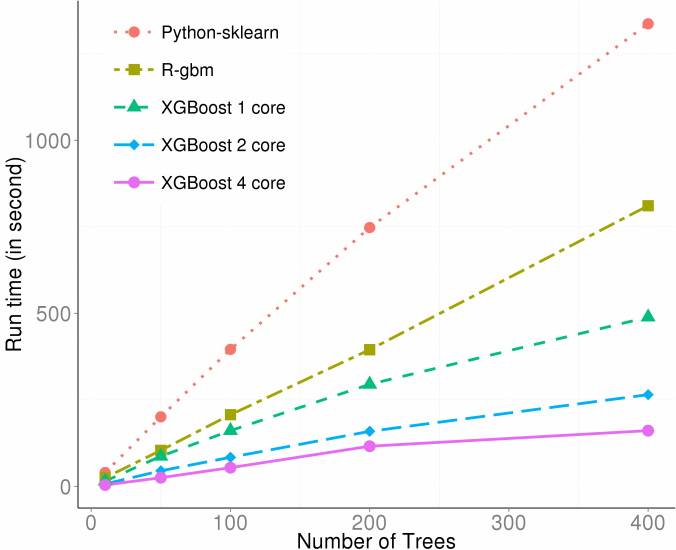
\includegraphics[width=.6\textwidth]{images/More/perf_un}
		\caption{Comparaison des temps d'apprentissage entre XGBoost et d'autres algorithmes importants de Machine Learning sur le challenge Kaggle du boson de Higgs}
		\label{fig:perfun}
	\end{margincap}
\end{figure}

Sur la Figure~\ref{fig:perfun}, les courbes \textit{Python-sklearn} et \textit{R-gbm} correspondent à des algorithmes GBM déjà existants sur ces plateformes, alors que XGBoost correspond à des essais avec l'algorithme nouvellement développé. L'influence du nombre de c\oe urs utilisés est également testé ici (tous les apprentissages se font à même paramétrage). On tire de ce graphe les conclusions suivantes :\begin{itemize}
\itemperso{XGBoost et autres GBM}Mis à part pour un faible nombre d'arbres appris, XGBoost obtient des performances de bien meilleures (deux fois plus rapide) que les autres solutions de GBM.
\itemperso{Influence du nombre de c\oe ur}Plus le nombre de c\oe urs pour paralléliser XGBoost est important, plus ce dernier est rapide, même si on observe un tassement passé quatre c\oe urs\mysidenote{Ceci est logique, car comme nous l'avons vu, il n'est pas possible de paralléliser tout le processus d'apprentissage, mais seulement une partie de ce dernier. Ainsi, il restera une partie que l'on ne peut réduire, d'où ce constat.}.
\end{itemize}

\subsubsection{Benchmarking par rapport à des implémentations de Random Forest}
Un autre Benchmarking a également visé à comparer les performances de XGBoost 

\subsection{Valeurs manquantes}
Les valeurs manquantes sont un problème courant en analyse de données. La plupart des algorithmes proposent aujourd'hui deux solutions, soit l'utilisateur pré-traite ses données avant de les utiliser et retire ou modifie au besoin les données manquantes, soit il \og laisse faire\fg{} l'algorithme, au risque que la solution ne lui convienne pas.

XGBoost se démarque ici en proposant un traitement non binaire (ie. on n'assigne pas par défaut \texttt{null} ou \texttt{0},...) pour traiter les données manquantes. À la place, l'algorithme propose d'assigner une direction aux valeurs manquantes plutôt qu'une valeur numérique particulière.

Ceci signifie que lorsqu'une découpe est réalisée selon une variable proposant des valeurs manquantes, l'algorithme va classer les données manquantes \og à gauche ou à droite\fg{} dans les fils du n\oe uds. A posteriori de ce classement, XGBoost va regarder quel classement fournirait le meilleur gain et re-répartir ces instances de manière à maximiser ce dernier\mysidenote{Pour les personnes intéressées, l'algorithme explicite est précisé dans l'article de T. \textsc{Chen} (Algorithme 3) \cite{bib:xgboost-article}}.

Ce comportement est activé par défaut pour XGBoost, et a pour intérêt que l'algorithme va apprendre une direction optimale au lieu de simplement considérer toutes les valeurs inconnues comme identiques ou alors les rejeter.
\subsection{Cross-validation native}
Pour simplifier l'utilisation de XGBoost, et uniformiser l'utilisation de cette dernière avec XGBoost, les auteurs des packages ont inclus une fonction de cross-validation directement dans XGBoost.

Cette dernière permet alors de reprendre tous les paramètres disponibles par XGBoost en apprentissage pour la cross-validation et d'avoir ainsi un fonctionnement continu. On retrouve en particulier la possibilité d'utiliser une fonction de perte personnalisée\mysidenote{Plus de détails sur les paramètres de XGBoost seront proposés en Section~\ref{sec:params}, on peut également trouver un descriptif de tous les paramètres en cross-validation à \cite{bib:cv-params}.}.


\section{Mise en \oe uvre}
\subsection{Grandes étapes de développement de XGBoost}
\label{sec:historique}
Comme tout projet informatique, XGBoost a été codée de manière itérative afin de s'adapter aux besoins des utilisateurs. Nous allons donc voir ici quelles sont les grandes étapes de développement de cette méthode et quels sont les objectifs futurs\mysidenote{L'historique qui vous sera proposé ici est issue de données récoltées dans les \textit{Release Note} de la page Git Hub du projet~\cite{bib:xgboost-git}, mais aussi d'un retour sur expérience du fondateur de XGBoost sur sa page personnelle~\cite{bib:xgboost-author}.}.

\subsubsection{Premières implémentations}
L'origine de la méthode provient de recherches de T. \textsc{Chen} sur le boosting d'arbres. L'auteur n'ayant pas trouvé de soution lui convenant, il a décidé d'implémenter sa propre solution et d'en faire un package \og maison\fg. Afin d'optimiser les performances, ce premier code a été réalisé en C++ en utilisant la librairie OpenMP pour avoir une parallélisation automatique sur les CPU multi-threads~\cite{bib:boson}.

Ce package a alors été utilisé sur le challenge Kagle \textit{Higgs Boson Challenge} et ses résultats ont été parmis les meilleurs et ont permis à d'autres concurrents d'améliorer leurs résultats.\mysidenoteoffset{-3cm}{En plus du développement accéléré de XGBoost suite à ce succès, son auteur a également publié un article de recherche précisant ses motivations, les modèles utilisés, et introduisant son code et ses algorithmes à la communauté~\cite{bib:boson}.}\mysidenoteoffset{0cm}{Les excellents résultats de XGBoost sur cette compétition ont également eu pour conséquence que cette méthode soit vue comme une avancée majeure en termes d'outils utilisés dans la recherche physique. Ainsi, XGBoost s'est vue attribuée la \textit{High Energy Physics meets Machine Learning Award} pour cette contribution.}.

Face à ce succès, un wrapper Python a alors été mis en place ainsi qu'une API pour l'utilisation. On retrouve alors la première version sur le répertoire Git, qui date de mars 2014. La première version du module Python est elle fournie dès mais 2014.

Suite à cela, le code continue a être développé pour aboutir en septembre 2014 à un module R et un début de parallélisation pour le booster linéaire. De même, l'algorithme de calcul d'arbres est accéléré.

On se retrouve donc à cette étape avec les éléments de la Figure~\ref{fig:dev_un}.

\begin{figure}[h]
	\begin{margincap}
		\centering
	  	\resizebox{.98\textwidth}{!}{%
		\noindent%
\begin{tikzpicture}
  \matrix (pythonwrapper) [row sep=2.8mm,column sep=2.8mm] {
    \node (python) [fill=themeColor!25, draw, rectangle with rounded corners, minimum width=3cm] {XGBoost Python}; & \node [fill=bluenight!25, draw, rectangle with rounded corners, minimum width=3cm] (panda) {pandas/numpy};\\
    \node (xgboost) [fill=themeColor!25, draw, rectangle with rounded corners, minimum width=3cm] {XGBoost\phantom{y}}; & \\
  };
  \path let \p1=($(python.west)-(panda.east)$),
            \n1 = {veclen(\p1)}
            in node[fill=vertforet, text=white, rectangle with rounded corners, draw, above=of pythonwrapper.north, anchor=south, yshift=-1cm, minimum width=\n1] {\textbf{Utilisateurs Python}};
  \matrix (rwrapper) [row sep=2.8mm,column sep=2.8mm, right=.5cm of pythonwrapper.east, anchor=west] {
    \node (r) [fill=themeColor!25, draw, rectangle with rounded corners, minimum width=3cm] {XGBoost R\phantom{y}}; & \node [fill=bluenight!25, draw, rectangle with rounded corners, minimum width=3cm] (dataframe) {dataframe\phantom{y}};\\
    \node (xgboostdeux) [fill=themeColor!25, draw, rectangle with rounded corners, minimum width=3cm] {XGBoost\phantom{y}}; & \\
  };
  \path let \p1=($(r.west)-(dataframe.east)$),
            \n1 = {veclen(\p1)}
            in node[fill=vertforet, text=white, rectangle with rounded corners, draw, above=of rwrapper.north, anchor=south, yshift=-1cm, minimum width=\n1] {\textbf{Utilisateurs R\phantom{y}}};
\end{tikzpicture}}
		\caption{Première étape de développement de XGBoost (d'après~\cite{bib:xgboost-author})}
		\label{fig:dev_un}
	\end{margincap}
\end{figure}

Ainsi, fin 2014, XGBoost était accessible dans les deux principaux langages de Machine Learning, Python et R.

\subsubsection{Mise en place de la version distribuée}
Suite aux bons résultats dans de nouveaux challenges Kaggle et en pratique, la méthode continu à se développer. Ainsi, une release de mai 2015 permet d'instaurer les points suivants :\begin{itemize}
	\itemperso{YARN}Une version distribuée qui fonctionne avec YARN et permet de traiter des volumes de données directement liés au Big Data.
	\itemperso{HDFS}Enregistrement et chargement de données depuis HDFS.
	\itemperso{Utilisation mémoire}Une première version expérimentale de la gestion de mémoire externe est mise en place.
	\itemperso{Améliorations}De plus, des améliorations continues aux packages R et Python sont mises en place, notament sur la possibilité d'enregistrer et charger des modèles via ces langages. De plus, le wrapper pour SKLearn (plateforme Python) est terminé.
\end{itemize}
Ainsi, XGBoost s'est ouvert à l'univers du Big Data via YARN et HDFS, mais s'est aussi concentré sur la création d'une interface uniforme entre les principaux langages (Pyhton et R). Ceci a ensuite permis aux développeurs de se concentrer plus spécifiquement sur les performances. Dans ces principaux langages, les principaux éléments accesibles sont présentés de la Figure~\ref{fig:dev_deux}\mysidenoteoffset{4cm}{Dans cette figure, apparaît le terme de \og\textit{gridsearch}\fg. Il s'agit en fait d'une méthode permettant de rechercher des paramètres optimaux pour les algorithmes (pour les paramètres de XGBoost, voir la Section~\ref{sec:params}). Ceci montre donc qu'en optimisant l'interface avec Scikit Learn et R, on augmente ainsi les capacité de XGBoost en l'interfaçant convenablement avec des technologies efficaces et déjà en place.}.

\begin{figure}[h]
	\begin{margincap}
		\centering
	  	\resizebox{.98\textwidth}{!}{%
		\noindent%
\begin{tikzpicture}
  \matrix (pythonwrapper) [row sep=2.8mm,column sep=2.8mm] {
    \node (python) [fill=themeColor!25, draw, rectangle with rounded corners, minimum width=3.25cm, text width=3.25cm, align=center] {XGBoost Python}; & \node (xgboost) [fill=themeColor!25, draw, rectangle with rounded corners, minimum width=3.25cm, text width=3.25cm, align=center] {XGBoost\phantom{y}};\\
    \node [fill=bluenight!25, draw, rectangle with rounded corners, minimum height=1.5cm, minimum width=3.25cm, align=center, text width=3.25cm] (pgrid) {scikit-learn\\gridsearch}; & \node [fill=bluenight!25, draw, rectangle with rounded corners, align=center, minimum height=1.5cm, minimum width=3.25cm, text width=3.25cm] (papi) {API classification\\scikit-learn\phantom{g}};\\
  };
  \path let \p1=($(pgrid.west)-(papi.east)$),
            \n1 = {veclen(\p1)}
            in node[fill=vertforet, text=white, rectangle with rounded corners, draw, above=of pythonwrapper.north, anchor=south, yshift=-1cm, minimum width=\n1] {\textbf{Utilisateurs Python}};
  \matrix (rwrapper) [row sep=2.8mm,column sep=2.8mm, right=.5cm of pythonwrapper.east, anchor=west] {
    \node (r) [fill=themeColor!25, draw, rectangle with rounded corners, minimum width=3.25cm, text width=3.25cm, align=center] {XGBoost R\phantom{y}}; & \node (xgboostdeux) [fill=themeColor!25, draw, rectangle with rounded corners, minimum width=3.25cm, text width=3.25cm, align=center] {XGBoost\phantom{y}}; \\
    \node [fill=bluenight!25, draw, rectangle with rounded corners, minimum height=1.5cm, minimum width=3.25cm, text width=3.25cm, align=center] (rgrid) {R caret\\gridsearch}; & \node [fill=bluenight!25, draw, rectangle with rounded corners, minimum height=1.5cm, minimum width=3.25cm, text width=3.25cm, align=center] (radaptator) {Adaptateur caret XGBoost};\\
  };
  \path let \p1=($(r.west)-(xgboostdeux.east)$),
            \n1 = {veclen(\p1)}
            in node[fill=vertforet, text=white, rectangle with rounded corners, draw, above=of rwrapper.north, anchor=south, yshift=-1cm, minimum width=\n1] {\textbf{Utilisateurs R\phantom{y}}};
\end{tikzpicture}}
		\caption{Deuxième étape de développement de XGBoost, uniformisation des offres entre langages (d'après~\cite{bib:xgboost-author})}
		\label{fig:dev_deux}
	\end{margincap}
\end{figure}

\subsubsection{Refactoring, autres compatibilité et parallélisme}
Après avoir réalisé les interfaces avec R et Python et mis un premier pied dans le monde du Big Data et du parallélisme, les développements se sont axés pour compléter l'offre logiciel et améliorer la qualité de l'existant. Ainsi, depuis mai 2015, seulement deux nouvelles versions majeures ont été distribuées, mais étendant le pannel de possibilités.

\subParagraphe{Mise à jour de janvier 2016}
Cette mise à jour a terminé les travaux sur les libraires R et Python en corrigeant les principaux bugs et en ajoutant plus de possibilités en paramétrage. En particulier pour Python, l'installation est simplifiée via un support pour \texttt{pip}. De même, des compatibilités avec les \textit{Data Frames} de Panda ont été ajoutées.

Outre ces premiers usages, une API JAVA est également proposée et prête à l'emploi.

Enfin, cette mise à jour marque un point important du point de vue de la maintenance future en ajoutant des sécurté supplémentaires et des solutions d'intégration continue pour rendre plus robuste les futures étapes.

\subParagraphe{Mise à jour de juillet 2016}
Cette dernière mise à jour majeure se caractérise par un refactoring important de la librairie. En particulier, le code C++ est entièrement remanié pour utiliser la version C++11, ceci implique en particulier des changements dans la gestion de l'aléatoire ou encore la gestion des pointeurs (et les questions de sécurité liées).

Cette mise à jour contient ensuite un nombre important de changements ou d'amélioration pour divers langages :
\begin{itemize}
	\itemperso{R}Possibilité d'utilisation des capacités de gestion de mémoire externe, ceci reste cependant toujours bloqué sous Windows pour cause de problèmes techniques.
	\itemperso{Multi-threading}Correctif pour rendre les librairies XGBoost et Rabit \textit{thread-safe}.
	\itemperso{JAVA}Un package spécifique pour JAVA et Scala est fourni, nommé XGBoost4j. La version JAVA distribuée fonctionne également sur les frameworks JAVA Flink et Spark.
\end{itemize}

Ces mises à jour montrent donc la réelle volonté actuelle pour XGBoost, qui est de pouvoir fonctionner sur diverses machines de manière distribuée, de manière transparente. Pour y arriver, un composant d'exécution pour faire le pont entre XGBoost et les différentes plateforme a été développé, du nom de Rabit. Son intérêt est illustré à la Figure~\ref{fig:dev_trois}.

\begin{figure}[h]
	\begin{margincap}
		\centering
	  	\resizebox{.98\textwidth}{!}{%
		\noindent%
\begin{tikzpicture}
  \matrix (platun) [row sep=2.8mm,column sep=2.8mm] {
    & \node (xgboosta) [fill=themeColor!25, draw, rectangle with rounded corners, minimum width=3cm, text width=3cm, align=center] {XGBoost}; \\
    \node (svma) [fill=vertforet!25, draw, rectangle with rounded corners, minimum width=3cm, text width=3cm, align=center] {SVM A}; & \node (rabbita) [fill=themeColor!25, draw, rectangle with rounded corners, minimum width=3cm, text width=3cm, align=center] {Abstraction Rabit};\\
  };
  \path let \p1=($(svma.west)-(rabbita.east)$),
            \n1 = {veclen(\p1)}
            in node[fill=vertforet, text=white, rectangle with rounded corners, draw, below=of platun.south, anchor=north, yshift=.9cm, minimum width=\n1] {\textbf{Plateforme A}};
 
  \matrix (platdeux) [row sep=2.8mm,column sep=2.8mm, right=.5cm of platun.east, anchor=west] {
    & \node (xgboostb) [fill=themeColor!25, draw, rectangle with rounded corners, minimum width=3cm, text width=3cm, align=center] {XGBoost}; \\
    \node (svmb) [fill=bluenight!25, draw, rectangle with rounded corners, minimum width=3cm, text width=3cm, align=center] {SVM B}; & \node (rabbitb) [fill=themeColor!25, draw, rectangle with rounded corners, minimum width=3cm, text width=3cm, align=center] {Abstraction Rabit};\\
  };
  \path let \p1=($(svmb.west)-(rabbitb.east)$),
            \n1 = {veclen(\p1)}
            in node[fill=bluenight, text=white, rectangle with rounded corners, draw, below=of platdeux.south, anchor=north, yshift=.9cm, minimum width=\n1] {\textbf{Plateforme B}};

  \matrix (plattrois) [row sep=2.8mm,column sep=2.8mm, right=.5cm of platdeux.south east, anchor=south west] {
    \node (xgboostc) [fill=themeColor!25, draw, rectangle with rounded corners, minimum width=3cm, text width=3cm, align=center] {XGBoost};\\
  };
  \node (singlema) [fill=violet, text=white, draw, rectangle with rounded corners, minimum width=3cm, text width=3cm, align=center, below=of plattrois.south, anchor=north, yshift=.9cm] {\textbf{Machine isolée}};\\
\end{tikzpicture}}
		\caption{Extension de XGBoost vers un système distribué transparent par le développement de Rabit (d'après~\cite{bib:xgboost-author})}
		\label{fig:dev_trois}
	\end{margincap}
\end{figure}

\subsubsection{Intégration dans des plateformes de machine learning}
En parallèle des développements \og officiels\fg{} de XGBoost, un certains nombre de plateformes de machine learning ont également annoncé intégrer XGBoost parmis les méthodes qu'elles proposaient à leurs utilisateurs. Ceci est le cas pour :
\begin{itemize}
	\itemperso{Data Science Studio}Il s'agit d'une plateforme de machine learning éditée par la société Dataiku. Cela permet ainsi à ses utilisateurs de pouvoir utiliser XGBoost sans avoir à rédiger (beaucoup) de code. Des exemples d'utilisation sont également fournis sur leur site~\cite{bib:xgboost-dataiku}. Cet ajout a été réalisé en août 2015.
	\itemperso{H2O.ai}Le 28 janvier 2017, le CTO de la société H2O.ai annonce sur les réseaux sociaux que l'algorithme XGBoost sera utilisable dans leur plateforme lors de la prochaine release majeure~\cite{bib:xgboost-hdeuxo}.
\end{itemize}
Ces deux exemples tendent à montrer que la méthode requiert l'intérêt de la communauté, et ce très tôt (mi-2015), ce qui peut être un bon indicateur de pérénité.

\subsubsection{Résumé}
En résumé de ces avancées, T.~\textsc{Chen} estime que le développement de XGBoost s'est fait sur le même modèle que celui d'Unix, à savoir être \og \textit{ouvert et s'intégrant bien aux autres systèmes par une interface commune}. Son idée est résumée de la manière suivante~\cite{bib:xgboost-author} :


\vspace*{.2cm}
\noindent\hspace*{\fill}\tikz{%
  \node (def_larousse) [color=mygray, align=justify, text width=.8\textwidth] at (0,0) {\textit{XGBoost was designed to be closed package that takes input and produces models in the beginning. The XGBoost package today becomes fully designed to be embeded into any languages and existing platforms. It is like a Lego brick, that can be combined with other bricks to create things that is much more fun than one toy.}};%
  \fill [\currentColor] ([xshift=-.15cm]def_larousse.north west) rectangle ([xshift=-.25cm]def_larousse.south west);%
}\hspace*{\fill}\vspace*{.2cm}

\subsection{Les paramètres}
L'implémentation de XGBoost laisse comme nous l'avons déjà laissé supposer propose un nombre important de paramètres laissés libres à l'utilisation. Ces paramètres peuvent être regroupés en trois familles que nous détaillerons tour à tour dans cette section.
\subsubsection{Paramètres génériques}
Ces paramètres permettent de définir les grandes lignes de l'algorithme, comme la version de boosting utilisée et des aspects plus \og administratifs\fg. Trois paramètres principaux sont proposés.

\subParagraphe{\texttt{Booster}}Il définit le type de boosting à employer pour l'entraînement du modèle. Nous avons présenté en Section~\ref{sec:gradient-boosting} la version de boosting associé aux arbres.
\subParagraphe{\texttt{Silent}}Ce mode permet de préciser si l'on demande lors de l'entraînement l'affichage d'informations dans la console (il s'agit en fait d'un mode \textit{verbose}).
\subParagraphe{\texttt{Nthread}}Ce paramètre permet de limiter le nombre de threads que l'algorithme va utiliser. En effet, comme nous l'avons évoqué à la Section~\ref{} cette méthode est optimisée pour utiliser au mieux les capacités de calcul de la machine.

\subParagraphe{Valeurs usuelles}Les valeurs communes et celles par défaut associées à ces paramètres sont listées à la Table~\ref{tab:params-generiques}.

\begin{table}[h]
  \begin{margincap}
    \centering
    \begin{tabular}[\margincapalign]{p{.2\textwidth}p{.4\textwidth}p{.3\textwidth}}
	\toprule
	\textbf{Paramètres}& \textbf{Valeurs} & \textbf{Par défaut} \\
	\midrule
	\texttt{booster}  & \texttt{gbtree} (arbres)\newline\texttt{gblinear} (linéaires) & \texttt{gbtree} \\
	\texttt{silent}   & \texttt{1} (activé)\newline\texttt{0} (non activé)& \texttt{0}\\
	\texttt{nthread}  & Valeur numérique & Rien, ie. le nombre maximum de threads disponibles. \\
	\bottomrule
    \end{tabular}
	\sidecaption{Valeurs pour les paramètres génériques de XGBoost}
	\label{tab:params-generiques}
  \end{margincap}
\end{table}
D'autres paramètres existent pour rendre la liste exhaustive. Pour plus de détails sur ces paramètres restants XXX.

\subsubsection{Paramètres de Boosting}
Comme nous l'avons vu à la Table~\ref{tab:params-generiques}, il existe différents types de Boosting que peut utiliser XGBoost. Dans la continuité des points abordés, nous nous attarderons plus en détail sur le paramétrage du booster à base d'arbres\mysidenote{La liste de paramètres ici proposée n'est pas exhaustive, nous avons cependant retenu les plus importants et ceux les plus souvent mis en avant lors des exemples d'utilisation de XGBoost. Pour une liste plus complète de ces paramètres, vous pouvez vous référer à~\cite{bib:params}.}. Ce choix est également motivé dans la mesure où ce dernier est le plus utilisé. On retrouve ici la partie la plus importante des paramètres pour XGBoost, et en particulier ceux permettant de contrôler le sur-apprentissage par le modèle.

\subParagraphe{\texttt{Eta}}Ce paramètre permet de contrôler le taux d'apprentissage (ie. un \og pas d'apprentissage\fg). Il permet en particulier d'augmenter la robustesse du modèle en diminuant les poids à chaque itérations.
\subParagraphe{\texttt{Min\_child\_weight}}Il définit une somme minimale pour les scores des observations d'une feuille après apprentissagemysidenote{Attention, il ne s'agit pas de compter le nombre d'observations par feuilles, mais les poids de ces observations.}. Ce paramètre étant fortement lié aux questions de sur-apprentissage, il est conseille de l'entraîner en utiliser la cross-validation proposée avec XGBoost.
\subParagraphe{\texttt{Max\_depth}}La profondeur maximale des arbres qui peuvent être appris. Comme pour \texttt{min\_child\_weight}, ce paramètre est lié au sur-apprentissage, il est donc conseiller de le choisir en utilisant la cross-validation.
\subParagraphe{\texttt{Max\_leaf\_nodes}}Il s'agit d'une version \og duale\fg{} du paramètre \texttt{max\_depth}, qui au lieu de contrôler la profondeur de l'arbre va contrôler le nombre de feuille terminale autorisées\mysidenote{Les arbres créés sont binaires, la correspondance est donc parfaite. Ainsi, un arbre de profondeur $p$ produira au maximum $2^p$ feuilles.}. Si jamais ce paramètre est défini, l'algorithme ne prendra pas en compte de valeurs pour \textt{max\_depth}. La même remarque s'applique quant à la manière de fixer sa valeur.
\subParagraphe{\texttt{Gamma}}L'intérêt est ici de fixer une valeur seuil pour autoriser la découpe d'un n\oe uds en deux sous-n\oe uds basé sur un critère de gain. Ce paramètre est le $\gamma$ observé dans la relation (\ref{eqn:gain}), et permet donc de définir le taux de laxisme pour la division des n\oe uds. De même, sa valeur dépendra fortement de la fonction de coût retenue, dans la mesure où le gain n'a pas d'unité absolue mais va dépendre de l'échelle imposée par la fonction de coût.

On rappelle que ce paramètre entre aussi en jeu dans la formule calculant la complexité d'un nouveau modèle, et est le paramètre lié au nombre de feuille de l'arbre (voir la relation (\ref{eqn:complexity_expr})).
\subParagraphe{\texttt{Lambda}}Il s'agit d'un terme de régularisation pour la norme imposée sur les c\oe fficients des feuilles dans le calcul de la complexité d'un arbre, comme observé avec la relation (\ref{eqn:complexity_expr}). Ce terme intervient aussi en régularisation dans le calcul du gain (\ref{eqn:gain}). Ce paramètre peut être utilisé en réduction du sur-apprentissage.
\subParagraphe{\texttt{Alpha}}Ce terme n'avait pas été abordé dans la partie théorique. Ce paramètre est analogue à \texttt{lambda}, il est cependant lié à norme un des poids\mysidenote{Il s'agit alors d'écrira la complexité sous la forme \[\Omega(f_t)=\gamma T+\frac{1}{2}\lambda\sum_{j=1}^T\omega_j^2+\alpha\sum_{j=1}^T|\omega_j|\]Le fonctionnement est alors analogue à celui d'une régression Lasso, avec une solution analytique qui n'existe pas, mais des solutions numériques possibles qui vont en plus faire de la sélection dans les paramètres.}. Comme pour une méthode de Lasso traditionnelle, utiliser ce paramètre permet de réduire le temps de calcul et est particulièrement bien adapté au contexte de hautes dimensions.
\subParagraphe{Subsample}Dans la mesure où l'algorithme va apprendre plusieurs modèles, l'idée est ici de sélectionner une partie (ou la totalité) de l'ensemble d'apprentissage et de renouveler ce pannel pour chaque modèle. On évite ainsi de trop coler à ces données.

\subParagraphe{Valeurs usuelles}La Table~\ref{tab:params-boosting} propose alors les valeurs possibles pour ces différents paramètres ainsi que les valeurs par défaut. Un paramètre numérique avec une valeur de \texttt{0} indique que ce dernier n'est pas utilisé par défaut.
\begin{table}[h]
  \begin{margincap}
    \centering
    \begin{tabular}{p{.3\textwidth}p{.4\textwidth}c}
	\toprule
	\textbf{Paramètres} & \textbf{Valeurs} & \textbf{Par défaut} \\
	\midrule
	\texttt{eta} & Conseillée entre \texttt{0.01} et \texttt{0.2}. & \texttt{0.3} \\
	\texttt{min\_child\_weight} & Valeur numérique & \texttt{1}\\
	\texttt{max\_depth} & Conseillé entre \texttt{3} et \texttt{10} & \texttt{6} \\
	\texttt{max\_leaf\_nodes} & Conseillé entre \texttt{8} et \texttt{1024} & \texttt{0} \\
	\texttt{gamma} & Valeur numérique & \texttt{0} \\
	\texttt{lambda} & Valeur numérique & \texttt{1} \\
	\texttt{alpha} & Valeur numérique & \texttt{0} \\
	\texttt{subsample} & Valeur <\texttt{1} & \texttt{1} \\
	\bottomrule
    \end{tabular}
	\sidecaption{Valeurs pour les paramètres liés au boosting d'arbre}
	\label{tab:params-boosting}
  \end{margincap}
\end{table}

\subsubsection{Paramètres d'apprentissage}
Pour terminer sur le détail des principaux paramètres de XGBoost, nous allons nous intéresser aux paramètres liés à l'apprentissage, c'est-à-dire pour la fonction objectif et les métriques utilisées. On retrouve trois grands axes.

\subParagraphe{\texttt{Objective}}Il s'agit de définir quel est la fonction de coût (la fonction $\ell$ dans la relation (\ref{eqn:loss_n})) à minimiser. Les calculs que nous avions proposés en Section~\ref{sec:gradient-boosting} supposait de prendre l'erreur MSE. Les trois solutions les plus communes sont :
\begin{itemize}
\itemperso{\texttt{linear}}Utilisation d'une simple fonction associée à la  régression linéaire (RMSE).
\itemperso{\texttt{logistic}}Pour des problèmes de classification binaire, il s'agit d'utiliser la fonction de régression logistique qui renvoie une probabilité d'appartenance à une classe.
\itemperso{\texttt{softmax}}Pour des problèmes de classification multiclasse, elle renvoie elle la classe prédite (et non une probabilité d'appartenance).
\itemperso{\texttt{softprob}}De même que pour \texttt{softmax} si ce n'est que l'on renvoie ici la probabilité.
\end{itemize}
\subParagraphe{\texttt{Eval\_metric}}Cette fonction peut être utilisée pour évaluer le modèle sur l'ensemble de test. À noter que si une fonction est précisée pour \texttt{objective} cette dernière sera nécessairement réutilisée. Des fonctions communes sont :
\begin{itemize}
\itemperso{\texttt{rmse}}Fonction d'erreur quadratique, utilisée couramment en régression.
\itemperso{\texttt{mae}}Fonction d'erreur absolue.
\itemperso{\texttt{logloss}}Utilisation de l'opposé de la log-vraissemblance.
\itemperso{\texttt{merror}}Une mesure de taux d'erreur pour le cas multiclasse.
\itemperso{\texttt{mlogloss}}Une utilisation de la log-vraissemblance pour le cas multiclasse.
\itemperso{\texttt{auc}}L'air sous la courbe ROC.
\end{itemize}
\subParagraphe{\texttt{\texttt{Seed}}}Un paramètre classique pour pouvoir \og figer\fg{} l'aléatoire entre deux implémentations et utilisations de l'algorithme. Cela permet donc de fournir des modèles reproductibles si nécessaire.

\subParagraphe{Valeurs usuelles}Pour conclure sur ce dernier ensemble de paramètre, nous précisons à la Table~\ref{tab:params-apprentissage} les valeurs usuelles et par défaut pour ces paramètres.
\begin{table}[h]
  \begin{margincap}
    \centering
    \begin{tabular}{p{.3\textwidth}p{.4\textwidth}c}
	\toprule
	\textbf{Paramètre} & \textbf{Valeurs} & \textbf{Par défaut} \\
	\midrule
	\texttt{objective} & \texttt{logistic} ; \texttt{softmax} ; \texttt{softprob} ; \texttt{linear} ; ...\newline Possibilité de fonction personnalisée& \texttt{linear} \\
	\texttt{eval\_metric} & \texttt{rmse} ; \texttt{mae} ; \texttt{logloss} ; \texttt{error} ; \texttt{merror} ; \texttt{mlogloss} ; \texttt{auc} ; ... & Variable\mysidenote{Comme nous l'avons déjà vu, cette valeur sera imposée si une valeur a été fournie à l'attribut \texttt{objective}.} \\
	\texttt{seed} & Valeur entière & \texttt{0} \\
	\bottomrule
    \end{tabular}
	\sidecaption{Valeurs usuelles et par défaut des paramètres pour l'apprentissage}
	\label{tab:params-apprentissage}
  \end{margincap}
\end{table}

\subsubsection{Prévenir le sur-apprentissage}
Comme nous l'avons mentionné, un certain nombre de paramètres sont à surveiller plus particulièrement. Nous regroupons ici les recommandations sur ces paramètres pour éviter les cas de sur-apprentissage.

Avant tout, il est bon de rappeler que le principe d'utiliser la régularisation pour XGBoost est déjà en soi un moyen de limiter ce sur-apprentissage. Cependant, il est nécessaire de biens configurer les paramètres associés comme nous allons le détailler ici.

\subParagraphe{Comment réduire le sur-apprentissage?}Dans le détail, l'algorithme XGBoost offre deux méthodes pour réduire le sur-apprentissage :
\begin{itemize}
\itemperso{Contrôle de la complexité}Cette dernière peut être contrôlée en contraignant les arbres qui seront générés. Les paramètres concernés sont ici \texttt{max\_depth}, \texttt{min\_child\_weight}, \texttt{max\_leaf\_node} et \texttt{gamma}.
\itemperso{Ajout d'aléatoire}Afin de rendre le résultat moins sensible au bruit. Deux solutions sont préconisées par les développeurs de XGBoost :
\begin{itemize}
\subitemperso{}Utiliser les paramètres influant sur l'ensemble d'apprentissage (\texttt{subsample} et \texttt{colsample\_bytree}\mysidenote{Ce paramètre n'avait pas été présenté auparavant. Son intérêt est de sélectionner aléatoirement des ensembles de colonnes en construisant les arbres afin d'introduire de l'aléatoire dans l'utilisation de ces dernières et éviter que tous arbres ne se ressemblent (on est proche de l'idée des Random Forest).}).
\subitemperso{}Réduire le pas d'apprentissage \texttt{eta} mais augmenter \texttt{num\_round}\mysidenote{Ce paramètre non présenté auparavant correspond au nombre d'étapes de Boosting a réaliser pour construire le modèle. L'idée est donc ici de l'augmenter pour contrebalancer la baise du pas d'apprentissage.} dans ce cas.
\end{itemize}
\end{itemize}
Les différents paramètres et la manière de déterminer leurs valeurs sera précisé dans les paragraphes qui suivent.

\subParagraphe{\texttt{min\_child\_weight}}En évitant d'apprendre des arbres avec des feuilles peu représentatives (ie. de poids faible), on se concentre sur l'apprentissage d'arbres plus représentatifs. Ainsi, des valeurs élevées permettent de prévenir l'apprentissage de relations trop spécifiques à l'ensemble utilisé pour les apprentissages.
\subParagraphe{\texttt{max\_depth}}De même, utiliser des arbres trop développés va entraîner que ces dernier soient trop spécifiques aux données des ensembles d'apprentissages, il est donc nécessaire d'utiliser des valeurs plus faibles.
\subParagraphe{\texttt{max\_leaf\_node}}Ce paramètre étant directement lié à \texttt{max\_depth}, la manière de l'appréhender est la même.
\subParagraphe{\texttt{subsample}}Pour éviter d'être trop spécifique vis-à-vis des données d'apprentissage, prendre des fractions différentes entre chaque arbre permet de moyenner les biais. Ainsi, prendre une fraction \og faible\fg{} de ces données est une option intéressante, il faut cependant faire attention à ce que la valeur ne soit pas trop basse, le risque étant alors d'être en sous-apprentissage en ne considérant pas assez de données.
\subParagraphe{\texttt{lambda}}Régulariser convenablement les scores des différentes feuilles peut permettre d'améliorer les problèmes de sur-apprentissage. Ainsi, bien que ce paramètre ne soit pas souvent utilisé, il est une option à considérer en cas de problème persistant.


\section{Applications}
\subsection{Challenges Kaggle}
\subsubsection{Apparition de XGBoost}
Comme cela a été expliqué, XGBoost est initiallement apparue lors d'un challenge Kaggle. Le challenge en question date de septembre 2014 et avait pour objectif d'explorer les apports possibles du Machine Learningpour la découverte de l'importance des expériences. En particulier, l'idée était la recherche possible de signal provenant de ces bosons à écarter d'un bruit important.

Le code utilisé était encore une version simple, mais qui a fourni un résultat capable de se classer parmis les 10\% les meilleurs\mysidenote{On pourra retrouver le code utilisé sur le répertoire Git de XGBoost~\cite{bib:xgboost-higgs}.}.

De plus, ces bons résultats ont conduits un nombre important de compétiteurs à tester cette solution qui a fini par être une des plus utilisées dans cette compétition.

Une présentation proposée post-challenge précise qu'il était ainsi possible se classer vers le vingt-cinquième rang de la compétition en utilisant un simple modèle XGBoost~\cite{bib:higgs-presentation}.

\subsubsection{Utilisations suivantes}
Par la suite, XGBoost a acquis une notoriété grandissante parmis les challengers de Kaggle et est aujourd'hui très largement diffusé dans cette communauté. Il entre ainsi dans la plupart des solutions obtenant de bons classements au côté d'autres méthodes comme les Random Forest. Des exemples marquants ont été regroupés dans la Table~\ref{tab:xgboost-kaggle}.

\begin{table}[h]
  \begin{margincap}
    \centering
    \begin{tabular}{ccp{.4\textwidth}c}
	\toprule
	    \textbf{Classement} & \textbf{Année} & \textbf{Challenge} & \textbf{Concurrent} \\
	\midrule
	2\up{nd} & 2017 & Allstate Claims Severity Competition & A. \textsc{Noskov} \\ 
	1\up{er} & 2016 & Knowledge Discovery and Data Mining Cup & V. \textsc{Sandulescu} \\
	1\up{et} et 3\up{ème} & 2015 & CERN LHCb experiment Flavour of Physics competition & V. \textsc{Mironov} \\
	1\up{er} & 2015 & Caterpillar Tube Pricing competition & M. \textsc{Filho} \\
	2\up{ème} & 2016 & AirBNB New User Bookings & N. \textsc{Kuroyanagi} \\
	2\up{ème} & 2016 & Allstate Claims Severity & A. \textsc{Noskov} \\
	    10\% & 2014 & Higgs Boson Competition & T. \textsc{Chen} \\
	    \multicolumn{4}{c}{...} \\
	    \bottomrule
    \end{tabular}
	  \caption{Quelques résultats utilisant XGBoost lors de challenges Kaggle}
	  \label{tab:xgboost-kaggle}
  \end{margincap}
\end{table}
L'influence de XGBoost dans le milieu des challenges Kaggle peut se résumer ainsi :

\vspace*{.2cm}
\noindent\hspace*{\fill}\tikz{%
  \node (def_larousse) [color=mygray, align=justify, text width=.8\textwidth] at (0,0) {\textit{Sur les challenges Kaggle de 2015, 17 solutions gagnantes sur 29 utilisaient XGBoost.}};%
  \fill [\currentColor] ([xshift=-.15cm]def_larousse.north west) rectangle ([xshift=-.25cm]def_larousse.south west);%
}\hspace*{\fill}\vspace*{.2cm}

\subsection{Utilisation par des entreprises}
De manière générale, les entreprises ne vont préciser en détail quels sont les modèles qu'elles utilisent pour obtenir leurs performances. Il est ainsi assez difficile de savoir qui utilise XGBoost à partir de simples témoignages. Cependant, deux sources nous ont permis d'avoir quelques informations sur la diffusion de cette méthode au sein de ces structures :\begin{itemize}
\itemperso{La page officielle de XGBoost}Sur cette dernière, les auteurs ont recensés quelques cas d'application de XGBoost en entreprise, selon des échos ou des discussions avec des responsables.
\itemperso{Les sites d'annonces d'emplois}Si la plupart des entreprise ne donnent pas leurs modèles, elles vont cependant demander aux candidats de maîtriser certaines techniques, et on peut ainsi avoir une idée des secteurs utilisant cet ensemble de méthodes.
\end{itemize}
\subsubsection{Cas d'utilisation mis en avant par XGBoost}
Les quelques cas de la Table~\ref{tab:etps-xgboost} sont mis en avant sur la page Github de XGBoost

\begin{table}[h]
	\begin{margincap}
	\centering
	\begin{tabular}{p{.2\textwidth}p{.6\textwidth}}
		\toprule
		\textbf{Entreprise} & \textbf{Utilisation} \\
		\midrule
		Alibaba & Utilisation dans son produit ODPS Cloud Service. \\
		Tencent & Utilisation pour faire un choix de prédiction dans le publicités à proposer aux internautes. En particulier, l'équipe technique motive son choix par la facilité d'intégration et la clareté du design de XGBoost.\\
		Auto Home & L'utilisation est ici pour la publicité en ligne et son optimisation. \\
	\end{tabular}
	\caption{Cas d'utilisation de XGBoost en entreprise, mis en avant par l'équipe de XGBoost}
	\label{tab:etps-xgboost}
	\end{margincap}
\end{table}

En plus de ces entreprises, on retrouve des intégrations de XGBoost parmis les plateformes de Machine Learning comme Anaconda, Dataiku ou encore H2Oai.

\subsubsection{Entreprise détectée via les offres d'emploi}
En regardant les offres sur les sites LinkedIn ainsi que sur Indeed, nous avons pu mettre en avant les entreprises de la Table~\ref{tab:etps-sites}, classées par secteurs d'activité.

\begin{table}[h]
	\begin{margincap}
		\centering
		\begin{tabular}{p{.2\textwidth}p{.6\textwidth}}
		\toprule
		\textbf{Secteur} & \textbf{Entreprises} \\
		\midrule
		Banque, crédit et assurances & AXA, Younited Crédit, Chubb, American Family Insurance \\
		Éditeurs de jeux & Pretty Simple, Kinect \\
		Vente & Expedia, Magnetic, Nativo, Seldon Technologies \\ 
		Consultants et services & Sonsoft Inc, Service Titan, EDJ Analytics, Comma Soft, Intermont \\
		Réseaux & Sesco \\
		\bottomrule
		\end{tabular}
		\caption{Entreprises demandant des compétences dans l'utilisation de XGBoost pour certaines de leurs annonces}
		\label{tab:etps-sites}
	\end{margincap}
\end{table}

On retrouve donc la plupart des \og grands\fg{} secteurs d'activité, et on remarque la présence de quelques grandes entreprises comme AXA ou Expedia. De plus, la répartition géographique est assez homogène, avec des résultats en Asie, en Europe ou en Amérique.

\subsection{Applications au domaine médical}
Nous venons de voir avec la Table~\ref{tab:etps-sites} que certains entreprises situées dans l'assurance s'intéressaient à XGBoost. Ceci nous a conduit à nous intéresser à l'utilisation qui peut être faite de XGBoost en médecine.

Si encore une fois aucun exemple professionnel n'est ressorti, nous avons pu mettre en avant deux travaux de personnes indépendantes pour réaliser de l'analyse de données médicales avec XGBoost.

\subParagraphe{Amélioration du taux de non-présentation des patients}Ce cas d'application est issu d'un travail personnel qui fut présenté devant des gérants d'agences de santé, et n'a donc pas été réalisé qu'à des fins \og d'études\fg. 

L'idée est ici de détecter des patients qui auraient dû se rendre dans des centres de santé mais ne l'ont pas fait et n'ont ainsi pas été diagnostiqués avant que des symptômes graves ne se déclenchent. 

Dans l'article détaillé \cite{bib:noshow}, l'auteur décrit l'intégralité de son processus de traitement de données. Nous retiendrons pour notre part ici que le modèle utilisé est un simple modèle XGBoost, pour lequel une phase de préparation des données et de recherche des paramètres optimaux a été menée, notament en suivant les bonnes pratiques présentées en Section~\ref{sec:bonnes-pratiques}.

Le modèle obtenu fourni ici des taux de vrais positifs et vrais négatifs compris entre 90 et 92\%, ce qui est considéré comme bon dans le domaine par l'auteur de l'étude. De plus, ce modèle a permis à son auteur de dresser une carte des quartiers à risque concernant ces non-présentations, que nous fournissons en Figure~\ref{fig:noshow}.

\begin{figure}[ht]
	\begin{margincap}
		\centering
		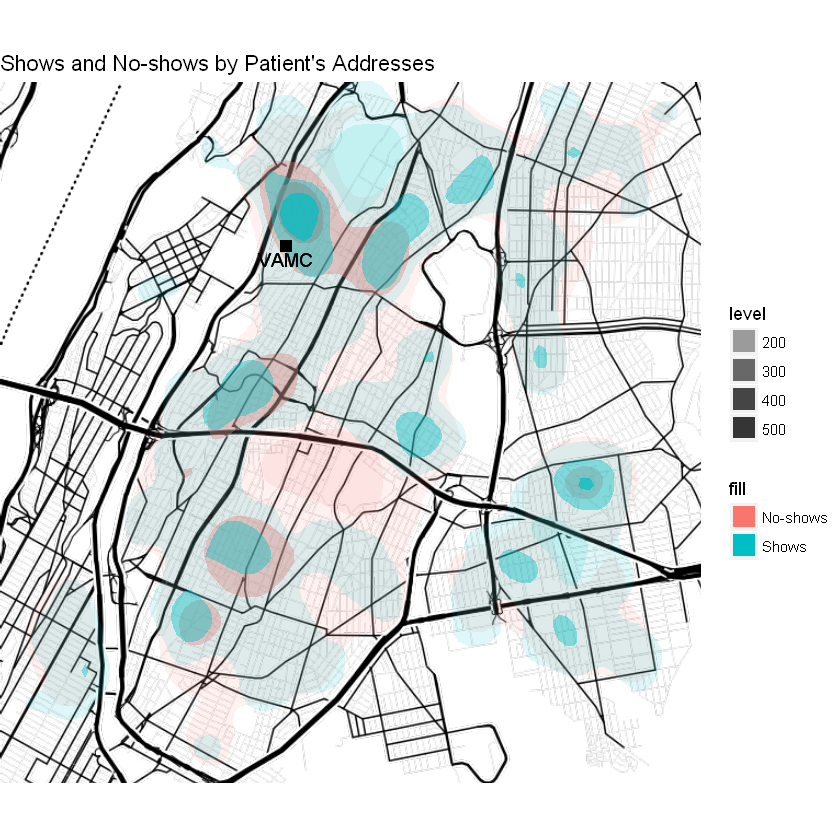
\includegraphics[width=.6\textwidth]{images/Applications/noshow}
		\caption{Carte de risque pour que les patients ne se présente pas au centre de soin établie à partir d'un modèle XGBoost.}
		\label{fig:noshow}
	\end{margincap}
\end{figure}

\subsubsection{Prévision de foyer de grippe}
Ce cas d'application (bien que beaucoup relayé sur Twitter) provient d'un membre de Github réalisant des essais de différentes méthodes de Machine Learning avec R. Dans le cadre de cet essai, l'idée était devoir s'il était possible de créer un modèle pour prévoir les morts dûs à la grippe H7N9 en Chine en 2013.

Après avoir fait des essais avec la plupart des méthodes classiques (Random Forest, Elastic Net et KNN entre autres), l'auteur s'est intéressée aux apports possibles de XGBoost à cette étude.

La conclusion est ici que XGBoot a permis d'obtenir des résultats avec moins d'imprécisions que l'ensemble des autres méthodes, et ce en utilisant les pratiques proposée à la Section~\ref{sec:bonnes-pratiques}\mysidenote{Le code fournit est assez complet, mais le conclusions peu détaillées, en particulier les notations utilisées pour la représentation des résultats. Le lecteur intéressé pourra cependant se rendre à la page en question \cite{bib:flue} pour de plus amples détails.}.



\section{Bonnes pratiques}
\label{sec:bonnes-pratiques}
En regardant les principaux tutoriels dédiés à l'utilisation de XGBoost, ainsi que les recommandations des auteurs de la méthode, il est possible d'en dégager un ensemble de bonnes pratiques. Nous allons présenter ces dernières dans cette partie.

Ces bonnes pratiques seront à avoir en tête lors de toute utilisation de XGBoost.

\subParagraphe{Fixer un niveau d'apprentissage élevé}
Pour mémoire, ce niveau d'apprentissage correspond au paramètre \texttt{eta}. Il est recommandé initialement de le fixer vers 0,1. Ce dernier sera ensuite affiné pour des valeurs entre 0,05 et 0,3 en fonction des données et des problèmes concernés.

L'idée est ici de prendre un niveau élevé (mais pas trop non plus!) afin que les apprentissages soient rapides et permettent de trouver les autres paramètres optimaux sans passer un temps (trop) considérable dans les phases d'apprentissage. Ainsi, une fois les autres paramètres correctement fixés, on pourra réduire le taux d'apprentissage pour affiner une dernière fois le modèle. On optimise ainsi le temps de configuration du modèle mais aussi ses performances.
\subParagraphe{Trouver le nombre optimal d'arbres}
Le nombre d'arbres est un des paramètres qui va le plus influer sur le temps d'apprentissage pour XGBoost, en effet, leur apprentissage est une tâche coûteuse et qui peut devenir inutile passé un certain stade (on observera des plateaux sur les performances au bout d'un certain moment).

À ce compte, il est conseillé d'utiliser les options de validation croisée automatiquement incluses dans XGBoost\mysidenote{Pour rappel, cette option va permettre de réaliser une validation croisée à chaque étape de boosting.}. Utiliser cette méthode va alors permettre de retourner le nombre optimal d'arbres \textit{in fine}.

\subParagraphe{Gérer les paramètres des arbres}Ces paramètres\mysidenote{Pour mémoire, il s'agit de \texttt{max\_depth}, \texttt{gamma}, \texttt{subsample}, \texttt{min\_child\_weight},...Pour revoir la signification de ces paramètres, voir la Section~\ref{sec:params-boosting}.} sont ceux qui auront le plus d'impact sur le modèle de sortie, comme pour le taux d'apprentissage, on partira de valeur élevée que l'on réduira au cours des itérations.

Il est aussi possible d'utiliser des solutions de \textit{grid search}\mysidenote{Par exemple en utilisant \texttt{GridSearchCV} en Python.} afin de trouver ces valeurs. Le temps de calcul peut alors courament avoisinner les 15 à 30 minutes (ou plus), ces opérations étant coûteuses.
\subParagraphe{Gérer les paramètres de régularisation}
Ces paramètres\mysidenote{Pour mémoire, il s'agit de \texttt{lambda} ou \texttt{alpha}, pour revoir leur signification, voir la Section~\ref{sec:params-boosting}.} vont permettre de simplifier le modèle tout en améliorant ses performances. On peut encore une fois utiliser des solutions de \textit{grid search} pour réaliser ce paramétrage.
\subParagraphe{Réduire le niveau d'apprentissage}Une fois les choix optimums réalisés pour les paramètres de régularisation ou d'arbres, on peut finir par affiner le taux d'apprentissage, comme nous l'avions expliqué initialement, afin d'optimiser une dernière fois notre apprentissage.
\subParagraphe{Utiliser l'AUC pour estimer les modèles}
Cette dernière recommandation ne vient pas réellement d'un paramètre, mais est un conseil générique, qui est de prendre l'aire sous la courbe ROC comme mesure par défaut pour les modèles, dans la mesure où cette dernière est souvent plus parlante que ne peut l'être la précision, le rappel,...

Ainsi, il est recommandé de l'utiliser, sauf en cas de besoins spécifiques\mysidenote{En particulier, nous avons vu comme XGBoost pouvait utiliser des fonctions de pertes personnalisées pour des cas plus exotiques à la Section~\ref{sec:perso-loss}.}.
\subParagraphe{Remarques générales}Enfin, un point comparable dans toutes les solutions proposées est que la recherche des paramètres optimaux va augmenter les performances, mais ne se suffit pas à elle-même. Ainsi, il est recommandé de l'utiliser en même temps que des solutions d'extraction de descripteurs pertinents, que l'utilisation de méthode dites \textit{Ensemble}\mysidenote{L'idée est ici d'avoir plusieurs modèles experts qui vont décider par vote majoritaire ou par moyenne.} ou encore de \textit{Stacking}\mysidenote{Il s'agit également d'une méthode permettant d'utiliser conjointement des modèles, un tutoriel basé uniquement sur ce point est disponible à~\cite{bib:stacking-kaggle}. De même, A. \textsc{Noskov}, classé seconde au \og\textit{Allstate Claims Severity Competition} (février 2017) a proposé une description de son modèle utilisant du stacking~\cite{bib:stacking-noskov}.}.


\section{Exemples}
\subsection{Utilisation basique}
Avant de regarder plus en détail des utilisations des fonctionnalités originales et avancées de XGBoost, nous fournirons ici quelques exemples d'utilisations de XGBoost avec les principaux langages sur lesquels il a été porté\mysidenote{Les différents exemples présentés proviennent directement de la documentation de XGBoost et présentent l'avantage de concerner le même jeu de données.}.

\subsubsection{En Python}
Tout le code nécessaire à l'utilisation de XGBoost est regroupé au sein du package développé mentionné dans l'historique de la Section~\ref{sec:historique}. 

\begin{lstlisting}[language=Python]
import xgboost as xgb

# Lecture des données
dtrain = xgb.DMatrix('demo/data/agaricus.txt.train')
dtest = xgb.DMatrix('demo/data/agaricus.txt.test')

# Paramètres spécifiés dans un dictionnaire
param = {'max_depth':2, 'eta':1, 'silent':1, 'objective':'binary:logistic'}
num_round = 2

# Création du modèle
bst = xgb.train(param, dtrain, num_round)

# Application du modèle en prédiction
preds = bst.predict(dtest)
\end{lstlisting}

\subsubsection{En R}
Tout le code nécessaire pour l'utilisation de XGBoost est ici aussi contenu dans un package nommé \texttt{xgboost}.

\begin{lstlisting}[language=R]
# Lecture des données
data(agaricus.train, package='xgboost')
data(agaricus.test, package='xgboost')
train <- agaricus.train
test <- agaricus.test

# Entrainement du modèle
bst <- xgboost(data = train$data, label = train$label, max.depth = 2, eta = 1, nround = 2, nthread = 2, objective = "binary:logistic")

# Application du modèle en prédiction
pred <- predict(bst, test$data)
\end{lstlisting}

\subsubsection{En Julia}

\begin{lstlisting}[language=julia]
using XGBoost

# Lecture des données
train_X, train_Y = readlibsvm("demo/data/agaricus.txt.train", (6513, 126))
test_X, test_Y = readlibsvm("demo/data/agaricus.txt.test", (1611, 126))

# Entrainement du modèle
num_round = 2
bst = xgboost(train_X, num_round, label=train_Y, eta=1, max_depth=2)

# Application du modèle en prédiction
pred = predict(bst, test_X)
\end{lstlisting}

\subsubsection{En Scala}

\begin{lstlisting}[language=Scala]
import ml.dmlc.xgboost4j.scala.DMatrix
import ml.dmlc.xgboost4j.scala.XGBoost

object XGBoostScalaExample {
  def main(args: Array[String]) {
    // Lecture des données
    val trainData =
      new DMatrix("/path/to/agaricus.txt.train")
    
    // Paramètres spécifiés dans une liste
    val paramMap = List(
      "eta" -> 0.1,
      "max_depth" -> 2,
      "objective" -> "binary:logistic").toMap
    val round = 2

    // Entrainement du modèle
    val model = XGBoost.train(trainData, paramMap, round)
    
    // Application du modèle en prédiction
    val predTrain = model.predict(trainData)
    model.saveModel("/local/path/to/model")
  }
}
\end{lstlisting}
\subsection{Utilisation avec Spark}
\begin{lstlisting}[language=Scala]
\begin{lstlisting}[language=Scala]
val spark = SparkSession.builder().appName("SimpleXGBoost Application").config("spark.executor.memory", "2G").config("spark.executor.cores", "4").config("spark.default.parallelism", "4").master("local[*]").getOrCreate()

// number of iterations
val numRound = 10
val numWorkers = 4
// training parameters
val paramMap = List(
      "eta" -> 0.023f,
      "max_depth" -> 10,
      "min_child_weight" -> 3.0,
      "subsample" -> 1.0,
      "colsample_bytree" -> 0.82,
      "colsample_bylevel" -> 0.9,
      "base_score" -> 0.005,
      "eval_metric" -> "auc",
      "seed" -> 49,
      "silent" -> 1,
      "objective" -> "binary:logistic").toMap
println("Starting Xgboost ")
val xgBoostModelWithDF = XGBoost.trainWithDataFrame(trainingData, paramMap,round = numRound, nWorkers = numWorkers, useExternalMemory = true)

val predictions = xgBoostModelWithDF.setExternalMemory(true).transform(testData).select("label", "probabilities")\end{lstlisting}
\end{lstlisting}
\subsection{Fonction de coût personnalisée}
\label{sec:cout-perso}
Nous avons à plusieurs reprise mentionné la possibilité d'utiliser les fonctions de pertes personnalisées avec XGBoost. Un exemple est fournit ci-dessous où l'on définit manuellement la fonction de log-vraissemblance pour la perte\mysidenote{La mesure de log-vraissemblance fait en réalité partie des options possibles par défaut dans XGBoost, elle est cependant présentée sous cette forme \og manuelle\fg{} ici à titre d'exemple. Pour mémoire, la manière de l'appeler serait de faire \texttt{objective = "binary:logistic".}}.

Cet exemple est réalisé en R, mais le fonctionnement sera le même pour d'autres langages.
\begin{lstlisting}[language=R]
loglossobj <- function(preds, dtrain) {
  # On extrait les labels de l'ensemble d'apprentissage
  labels <- getinfo(dtrain, "label")
  # Calcul du gradient et de la partie de la hessienne utiles 
  # dans les relations de boosting.
  preds <- 1/(1 + exp(-preds))
  grad <- preds - labels
  hess <- preds * (1 - preds)
  # Renvoie des résultats sous forme de liste.
  return(list(grad = grad, hess = hess))
}

# Entrainement du modèle avec notre méthode
model <- xgboost(data = train$data, label = train$label, nrounds = 2, objective = loglossobj, eval_metric = "error")
\end{lstlisting}

On remarque donc que la définition est des plus simples\mysidenote{Tant que l'on peut trouver des expressions algébriques...}, dans la mesure où les seuls éléments demandés sont de pouvoir exprimer le gradient et la hessienne de la fonction de perte.

\subsection{Sélection de variables}
Le dernier exemple d'application que nous proposerons ici est celui de la recherche d'importance des variables. En effet, certains algorithmes de Machine Learning (comme les Random Forest), peuvent permettre de comparer l'importance des variables entre elles.

Dans la mesure où XGBoost va à l'instar des Random Forest entraîner plusieurs arbres et faire des choix sur les variables les plus pertinentes pour créer de nouvelles branches, il est possible de mettre en place un calcul d'importance des variables via XGBoost. Ce calcul peut être réalisé en utilisant par exemple le code R suivant.
\begin{lstlisting}[language=R]
bst <- xgboost(data = train$data, label = train$label, max.depth = 2, eta = 1, nthread = 2, nround = 2,objective = "binary:logistic")
importance_matrix <- xgb.importance(agaricus.train$data@Dimnames[[2]], model = bst)
xgb.plot.importance(importance_matrix)
\end{lstlisting}
Ce code permet alors d'obtenir les évaluations de la Figure~\ref{fig:feature-importance}.

\begin{figure}[h]
	\begin{margincap}
		\centering
		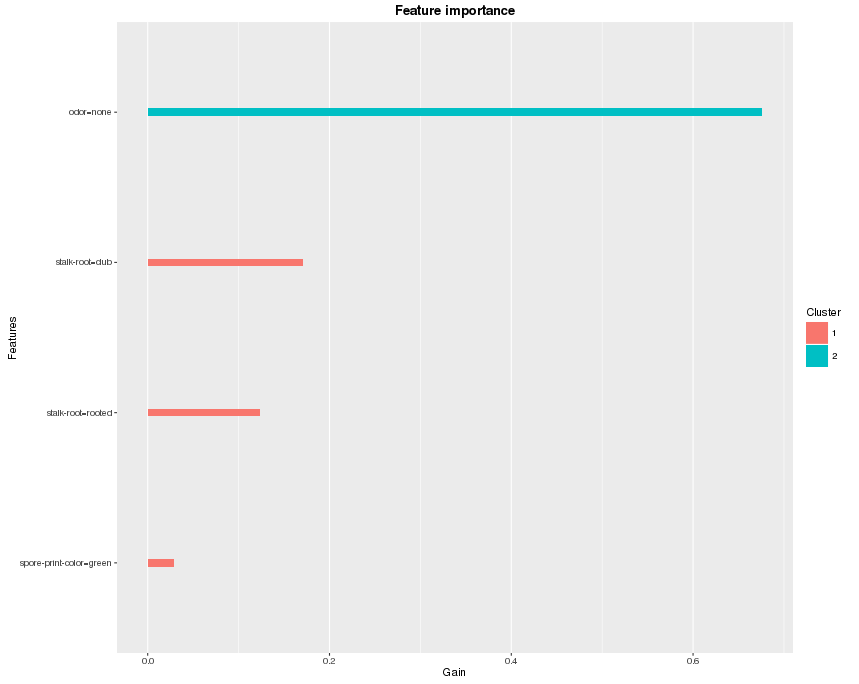
\includegraphics[width=.7\textwidth]{images/Exemples/feature-importance}
		\caption{Exemple d'affichage de l'importance des variables via XGBoost}
		\label{fig:feature-importance}
	\end{margincap}
\end{figure}

Dans ce cas particulier on remarque que la plupart de l'information est portée par le premier paramètre, les autres ne retenant qu'une part plus faible de cette dernière. En particulier, le dernier pourraît être supprimé de l'apprentissage, dans la mesure où il semble peu révélateur.

%\subsection{Comparaison de méthodes}

\section{Une solution d'avenir?}
Pour terminer sur ce panorama concernant XGBoost, nous allons tenter de répondre à la question suivante : \og XGBoost est-elle une solution vouée à perdurer?\fg.

Tout d'abord, comme nous l'avons vu, XGBoost est une méthode récente, dont la première implémentation remonte à trois ans. Nous avons cependant mis en avant le fait que cet algorithme a très vite été porté sur les principales plateformes et langages de Machine Learning. Il s'agit ainsi d'un premier point en faveur d'une perrenité de XGBoost, la méthode a été unanimement reconnue comme utile dans la communauté des \textit{data scientists} qui ont investi du temps pour l'intégrer à leurs écosystème. La finalisation de point étant en particulier un interfaçage complet avec le framework Haddop via une API unifiée JAVA/Scala.

Dans un second temps, nous avons également vu que même si les entreprises restent discrètes sur le sujet, des personnes ayant connaissance (et maîtrisant) XGBoost commencent à être recherchées par ces dernières. Ainsi, L'ancrage de XGBoost dans l'industrie est en train de s'opérer, ce qui est facteur très encourageant pour sa survie.

Enfin, les performances permises tant du point de vue des résultats en prédiction que des temps de calculs font de cette solution une méthode compétitive, y compris vis-à-vis des méthodes déjà bien implantées comme les Random Forest.

Tous ces éléments tendent à penser que XGBoost n'est pas qu'un \og effet de mode\fg, mais une méthode qui devrait s'installer durablement dans le domaine du Machine Learning, comme l'ont fait auparavant les Random Forest, les SVM,...Cependant, cette richesse a un coût, avec un algorithme demandant une certaine expertise dans sa configuration.

Pour terminer, nous pouvons également avancer que les développements \og bruts\fg{} de XGBoost arrivent à un degré de maturité importants, et se font donc moins importants. Ceci peut se voir dans le graphe de commits de la page Github de XGBoost, où on remarque que le volume de commits reste faible depuis un peu plus six mois, signe de la maturité du projet, qui est désormais de plus en plus intégré dans les plateformes, mais avec un code initial stable. Ce graphe vous est proposé à la Figure~\ref{fig:graphe-commits}.

\begin{figure}[h]
	\begin{margincap}
		\centering
		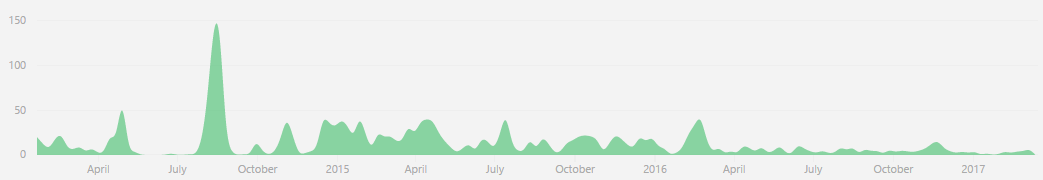
\includegraphics[width=\textwidth]{images/graphe-commits}
		\caption{Évolution du nombre de commits sur la page Github de XGBoostn établi en mars 2017}
		\label{fig:graphe-commits}
	\end{margincap}
\end{figure}


\nocite{*}
%\stepcounter{section}
%\addcontentsline{toc}{section}{Références}
\section{Références}
%\printbibliography
\begingroup
\renewcommand{\section}[2]{}%
\bibliographystyle{unsrt}
\bibliography{bib/xgboost}
\endgroup

%
% 3 - Ajout table des matières et liste des figures ; tables
%     Utilisation des préférence utilisateurs :
%          * \whereTOC -> end
%          * \whereLOF -> end
%          * \whereLOT -> end
%          * \TOCLOFTNumStyle -> via le fichier de conf xxx
%     Un réglage manuel comlémentaire est possible sur les \vfill - \newpage
%

\makeatletter
\ifnum\pdf@strcmp{\whereTOC}{end}=0
\clearpage
\else\ifnum\pdf@strcmp{\whereLOT}{end}=0
\clearpage
\else\ifnum\pdf@strcmp{\whereLOF}{end}=0
\clearpage
\fi\fi\fi

\includeTOC{end}
\includeLOF{end}
\includeLOT{end}

\end{document}
